\documentclass[12 pt]{report}
\usepackage[utf8]{inputenc}
\usepackage[french]{babel}
\usepackage[T1]{fontenc}
\usepackage{graphicx}
\usepackage{fancyhdr}
\usepackage[a4paper,left=2.5 cm,right=2 cm,top=2.5 cm,bottom=2.5 cm]{geometry}
\setlength{\parindent}{0 cm}
\setlength{\parskip}{1 ex plus 0.5 ex minus 0.2 ex}
\newcommand{\hsp}{\hspace{20 pt}}
\newcommand{\HRule}{\rule{\linewidth}{0.5 mm}}
\usepackage[Glenn]{fncychap}
\usepackage{setspace}
\setstretch{1.5}
 \usepackage{lmodern}
 \usepackage{enumitem}
 \usepackage{pifont}
 \usepackage[table,xllnames,dvipsnames,svgnames]{xcolor}
 \setcounter{secnumdepth}{4}
  \setcounter{tocdepth}{4}
  \usepackage{ragged2e}
\newlist{gitemize}{itemize}{4}
\setlist[gitemize,1]{
  leftmargin=\dimexpr0.3cm+\labelsep\relax,
  label={\smash{\raisebox{-0.25\height}{
\includegraphics[width=0.6cm]{Brackets_Icon.png}}}}
}
 \newlist{fitemize}{itemize}{4}
\setlist[fitemize,1]{
  leftmargin=\dimexpr0.3cm+\labelsep\relax,
  label={\smash{\raisebox{-0.25\height}{
\includegraphics[width=0.6cm]{800px-Visual_Studio_Code.png}}}}
}
 \newlist{hitemize}{itemize}{4}
\setlist[hitemize,1]{
  leftmargin=\dimexpr0.3cm+\labelsep\relax,
  label={\smash{\raisebox{-0.25\height}{
\includegraphics[width=0.8cm]{Xampp_logo.png}}}}
}
 \newlist{jitemize}{itemize}{4}
\setlist[jitemize,1]{
  leftmargin=\dimexpr0.3cm+\labelsep\relax,
  label={\smash{\raisebox{-0.25\height}{
\includegraphics[width=0.8cm]{HTML_logo.png}}}}
}
\newlist{kitemize}{itemize}{4}
\setlist[kitemize,1]{
  leftmargin=\dimexpr0.3cm+\labelsep\relax,
  label={\smash{\raisebox{-0.25\height}{
\includegraphics[width=0.8cm]{CSS3_logo_and_wordmark.png}}}}
}
\newlist{litemize}{itemize}{4}
\setlist[litemize,1]{
  leftmargin=\dimexpr0.3cm+\labelsep\relax,
  label={\smash{\raisebox{-0.25\height}{
\includegraphics[width=0.8cm]{bootstrap-4-the-most-popular-html-css-and-js-library.png}}}}
}
\newlist{mitemize}{itemize}{4}
\setlist[mitemize,1]{
  leftmargin=\dimexpr0.3cm+\labelsep\relax,
  label={\smash{\raisebox{-0.25\height}{
\includegraphics[width=0.8cm]{logo_javascript.png}}}}
}
\newlist{witemize}{itemize}{4}
\setlist[witemize,1]{
  leftmargin=\dimexpr0.3cm+\labelsep\relax,
  label={\smash{\raisebox{-0.25\height}{
\includegraphics[width=0.8cm]{1280px-PHP-logo.png}}}}
}
\newlist{xitemize}{itemize}{4}
\setlist[xitemize,1]{
  leftmargin=\dimexpr0.3cm+\labelsep\relax,
  label={\smash{\raisebox{-0.25\height}{
\includegraphics[width=0.8cm]{illu_ajax-et-l-echange-de-donnees-en-javascript.png}}}}
}
\newlist{citemize}{itemize}{4}
\setlist[citemize,1]{
  leftmargin=\dimexpr0.3cm+\labelsep\relax,
  label={\smash{\raisebox{-0.25\height}{
\includegraphics[width=0.8cm]{MySQL-Logo.png}}}}
}
\begin{document}

\includegraphics[width=16cm,height=22cm]{pdg.png}
\thispagestyle{empty}
\newpage
\thispagestyle{empty}
\begin{center}


\Huge\textbf{\fontfamily{lmtt}\selectfont {Dédicace}}
\end{center}


 A ceux qui méritent mes sincères remerciements et à qui je souhaite que Dieu les garde et leur réserve la santé et le bonheur, je trouve le plaisir de leur dédier ce modeste travail.
\\
\\
\begin{center}
\Large\fontfamily{pzc}\selectfont {A}\\
\Large\textbf{\fontfamily{pzc}\selectfont {Ma famille}}
\end{center}
 Qui dont- elle a fait preuve m’a appris ce que c’est la vie pour l’amour qu’elle m'a portée, pour le sacrifice, pour la confiance et la patience 

\begin{center}
\Large\textbf{\fontfamily{pzc}\selectfont {A}}\\
\Large\textbf{\fontfamily{pzc}\selectfont {Mes frères, mes amis et mes enseignants}}
\end{center}
 Pour leurs encouragements et leurs aides et surtout pour leur confiance.
Que ce travail soit à la hauteur de leur patience, témoigne ma connaissance et mon attachement indéfectible.
 
\newpage
\thispagestyle{empty}
\begin{center}
\Huge\textbf{\fontfamily{lmtt}\selectfont {Remerciement}}
\end{center}

\textbf{Au terme de mon projet de fin d’études, je tiens à adresser mes plus vifs remerciements à toutes les personnes qui, de près ou de loin, ont contribué à l’aboutissement de ce travail dans les meilleures conditions.}
 \\
 
 \textbf{Je remercie vivement les membres du jury que je remercie d’avoir accepté d’évaluer ce projet.}
 \\

\textbf{pour la qualité de l’encadrement qu’elle m’a assurée, pour sa disponibilité, ses conseils et remarques judicieuses et surtout pour sa confiance et ses encouragements continuels qui m’ont permis d’avancer.} 
\\

\textbf{Enfin, nous sommes reconnaissants à tout le personnel et le corps professoral de l’ISIGK et à tous ceux qui nous ont apporté de l’aide même minime.}
  

\fancypagestyle{plain}
{
    \fancyhead{}
    \fancyfoot{}
}
 \renewcommand\thepage{}
\tableofcontents
\renewcommand\thepage{\arabic{page}}  
\fancypagestyle{plain}
{
    \fancyhead{}
    \fancyfoot[C]{\thepage}
}
\renewcommand\thepage{}
\newpage
\renewcommand\thepage{\arabic{page}}  
\fancypagestyle{plain}
{
    \fancyhead{}
    \fancyfoot[C]{\thepage}
}
\renewcommand\thepage{}
\listoffigures
\renewcommand\thepage{\arabic{page}}  
\fancypagestyle{plain}
{
    \fancyhead{}
    \fancyfoot[C]{\thepage}
}
\renewcommand\thepage{}
\newpage
\renewcommand\thepage{\arabic{page}}  
\fancypagestyle{plain}
{
    \fancyhead{}
    \fancyfoot[C]{\thepage}
}
\newpage

\newpage
\renewcommand\thepage{}
\listoftables
\thispagestyle{empty}
\newpage
\renewcommand{\thepage}{\arabic{page}}
\setcounter{page}{1}
\chapter*{Introduction générale}  
\addcontentsline{toc}{chapter}{Introduction générale} 

 De nos jours, les organisations connaissent de perpétuels changements (restructurations, évolutions de métiers, mutations technologiques…). D’autre part, des nombreuses universités migrent de plus en plus vers les systèmes informatiques centralisés au détriment de leurs systèmes de gestion de bases de données traditionnels. Le besoin en matière d’accès aux informations est devenu pressant pour permettre aux utilisateurs de gérer et de suivre tout ce qui rapporte à l’université.
\\

Ces systèmes d’informations se révèlent un vecteur de performance essentiel pour la productivité de l’institut puisqu’ils sont des outils logiciels de pilotage de l’activité départementale et administrative, permettant à une université, et en particulier l’ISIGK, de gérer et d’optimiser cette activité.
\\

En effet, les activités administratives au sein d’un institut sont diverses (gestion des rattrapages, gestion des absences des enseignants, gestion des congés, …) et gérés par plusieurs employés (enseignants, employés administratif…). Donc, il est important d’améliorer le système informatique existant afin de corriger ses lacunes
\\

Sur le marché de logiciels, ces genres de systèmes informatiques existent d’une manière indépendante, c'est-à-dire que pour chaque activité au sein de l’institut un logiciel spécifique le gère. Ce qui est remarqué qu’il y a des tâches qui sont faits d’une manière manuelle telle que la suppression des absences des enseignants après qu’ils sont faits des rattrapages et l’ajout des données des enseignants remplaçants, qui amène à une redondance des données, difficultés à manipuler les informations et un travail répétitif qui mène à une perte de temps.
 \\
 
D’où l’importance de développer un système informatique qui traite ces lacunes.
\\

C’est dans ce cadre que s’intègre notre projet de fin d’étude qui s’est déroulé au sein de l’Institut Supérieur d’Informatique et de Gestion, établissement universitaire situé à Kairouan.
\\

De ce fait, notre objective visait à mettre en œuvre une solution logicielle intégrée et hautement paramétrable pour la gestion des rattrapages et d’absence qui souscrit les différentes opérations demandées par l’institut.
\\

Notre solution doit être puissante et souple à la fois, permettant d’organiser le travail.


\newpage
\chapter{État de l'art}
\section*{Introduction}  
\addcontentsline{toc}{section}{Introduction}
Dans un premier chapitre, nous présentons l’organisme d’accueil où nous avons effectué notre stage de fin d’études, tel que le système existant avec ses différentes problématiques.
Puis, nous proposons une solution. Enfin, nous dérivons la méthodologie de développement que nous avons adopté en argumentant notre choix.
\section{Présentation d’entreprise d’accueil }

\textbf{ L'Institut supérieur d'informatique et de Gestion de Kairouan (ISIGK) }est un établissement universitaire tunisien rattaché à l'Université de Kairouan et placé sous la tutelle
du ministère de l'enseignement supérieur et de la recherche scientifique.
\\

L’Institut Supérieur d’Informatique et de Gestion de Kairouan est installé a Avenue
Khemais El Alouini - 3100 Kairouan Elle a été fondée en 2002.
\\
Elle se compose de deux parties :
\\
\begin{itemize}[font=\color{Indigo} \Large, label=\ding{69}]
\item La partie administrative composée par les employés de l’institut est guidé par un
secrétaire générale, tout ayant le rôle de s’occuper des procédures et des règlements des
membres. 
\item Les parties Pédagogiques composées par les professeurs répartis dans les deux
départements de Gestion et de Informatique ayant chacun un chef de département. 

\end{itemize}
\begin{itemize}[font=\color{Indigo} \Large, label=\ding{68}]

\item\textbf{Diplômes :}




\begin{itemize}[font=\color{Indigo} \Large, label=\ding{67}]
\item Licences appliquées :


\begin{itemize}[font=\color{Indigo} \Large, label=\ding{66}]

	\item E-services
	\item Comptabilité : techniques comptables et financières
	\item Technologie des réseaux informatiques
	\item Économie et finance internationale : banques et assurances
	\item Marketing : e-marketing

\end{itemize}
\item Licences fondamentales:
\begin{itemize}[font=\color{Indigo} \Large, label=\ding{66}]

\item Sciences de l'informatique
\item Gestion : gestion d'affaires
\end{itemize}
\end{itemize}
\item \textbf{Organigramme :}	
la figure suivante représente l'organigramme de l'institut supérieur d'informatique et de gestion du Kairouan:
\end{itemize}
\begin{figure}[h]
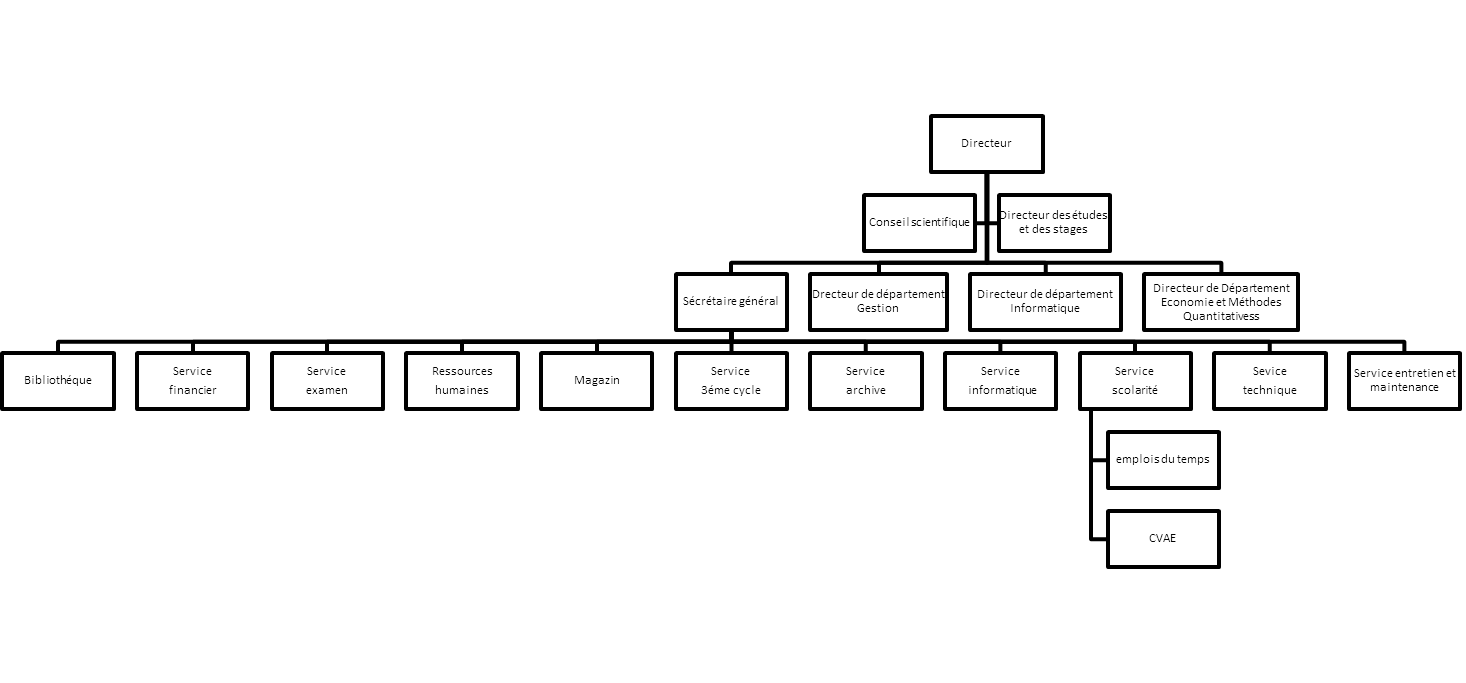
\includegraphics[height=8cm]{Organigramme.png}
\caption{ Organigramme de l'ISIGK}
\end{figure}
\newpage

\section{Présentation de l’existant }

L’étude de l’existant est une phase importante pour bien comprendre le système actuel et définir ses objectifs. L’établissement utilise des méthodes informatisées dont dans un premier lieu elles présentent certaines lacunes et dans deuxième lieu elles sont parfois des méthodes primitives (Excel…). 
\section{Critique de l’existant }
Il y a toujours des problèmes, en particulier lorsqu’un enseignant était absent et il voudra faire des rattrapages dans le but de l'éliminer, la suppression de ces absences ce fait d’une manière manuelle ,aussi la demande de rattrapage par les enseignants  se fait par téléphone, en outre, lorsqu’un enseignant demande un congé, il détermine seulement le type du congé sans préciser la période demandée qu’elle est mise par le personnel dont il nécessite un remplaçant, les données relatives à ce dernier ne sont pas ajoutées à la base des données de l’institut. 
Ce qui provoque des difficultés dans le déroulement du travail au sein de l’ISIGK, de plus, nous remarquons qu’il y a un gaspillage du temps.    

\section{Présentation du sujet proposé }
\subsection{Problématique }
\begin{itemize}[font=\color{black} \Large, label=\ding{55}]
\item La plateforme au sein de l'ISIGK est déjà existante mais elle possède beaucoup des lacunes, citons :
\begin{itemize}[font=\color{red} \Large, label=\ding{56}]

	\item Lorsqu’un personnel organise un rattrapage pour un enseignant, la suppression des absences de ce dernier après qu'il fait son rattrapage se fait manuellement.
	\item L'affectation  des données des enseignants remplaçants dans la base ne fera pas.
	\item la demande des rattrapages est faite par téléphone.

	\item La mauvaise visibilité et organisation des rattrapages.
\end{itemize}
\end{itemize}
\subsection{Solution envisagée}
\begin{itemize}[font=\color{black} \Large, label=\ding{51}]
\item Puisque nous ne pouvons pas accéder au code source de l’ancienne plateforme nous sommes obligées de développer une nouvelle application web-mobile qui traite ses lacunes dont elle offre la possibilité de : 
\begin{itemize}[font=\color{green} \Large, label=\ding{52}]

	\item 	Supprimer les absences des enseignants après que le rattrapage est fait d’une maniéré automatique.
	\item 	Affecter les enseignants remplaçants d’une maniéré automatique.
	\item Ajouter les rattrapages d'une façon correcte et automatique.
	\item 	Rendre la visibilité plus claire 
\end{itemize}
\end{itemize}
\section{Méthodologie de travail adoptée }
Afin d’éviter de se lancer d’une manière quelconque dans le développement de ce projet et se trouver à la suite, coincé à la moindre complication, nous avons opté pour le choix d’un modèle de développement.
\subsection{  Méthode de modélisation }
Pour le cas de notre application, et vu à la nature du projet, nous avons décidé de suivre le modèle Processus Unifié.
\subsubsection{Principe}
Le processus unifié est un processus de développement logiciel itératif, centré sur l'architecture, piloté par des cas d'utilisation et orienté vers la diminution des risques. C’est un patron de processus pouvant être adaptée à une large classe de systèmes logiciels, à différents domaines d'application, à différents types d'entreprises, à différents niveaux de compétences et à différentes tailles de l'entreprise.
\newpage
\begin{itemize}[font=\color{black} \Large, label=\ding{75}]
\item Itératif:
L'itération est une répétition d'une séquence d'instructions ou d'une partie de programme un nombre de fois fixé à l'avance ou tant qu'une condition définie n'est pas remplie, dans le but de reprendre un traitement sur des données différentes. Elle qualifie un traitement ou une procédure qui exécute un groupe d'opérations de façon répétitive jusqu'à ce qu'une condition bien définie soit remplie.
\\
la figure suivante représenter l'interaction du processus unifié.  
\begin{figure}[h]
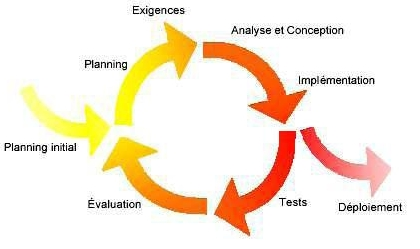
\includegraphics[height=10cm]{pic1.jpg}
\caption{L'itération du  processus unifié }
\end{figure}
\\

\item Le processus unifié  est piloté par les cas d'utilisation d'UML :
 \\
Le but principal d'un système informatique est de satisfaire les besoins du client. Le processus de développement sera donc accès sur l'utilisateur. Les cas d'utilisation permettent d'illustrer ces besoins.
Ils détectent puis décrivent les besoins fonctionnels (du point de vue de l'utilisateur), et leur ensemble constitue le modèle de cas d'utilisation qui dicte les fonctionnalités complètes du système.
\newpage
\item 	Le processus unifié  est centré sur l’architecture : 
\\
 la figure suivante représenter la centralisation du processus unifié sur l'architecture:

\begin{figure}[h]
\begin{center}
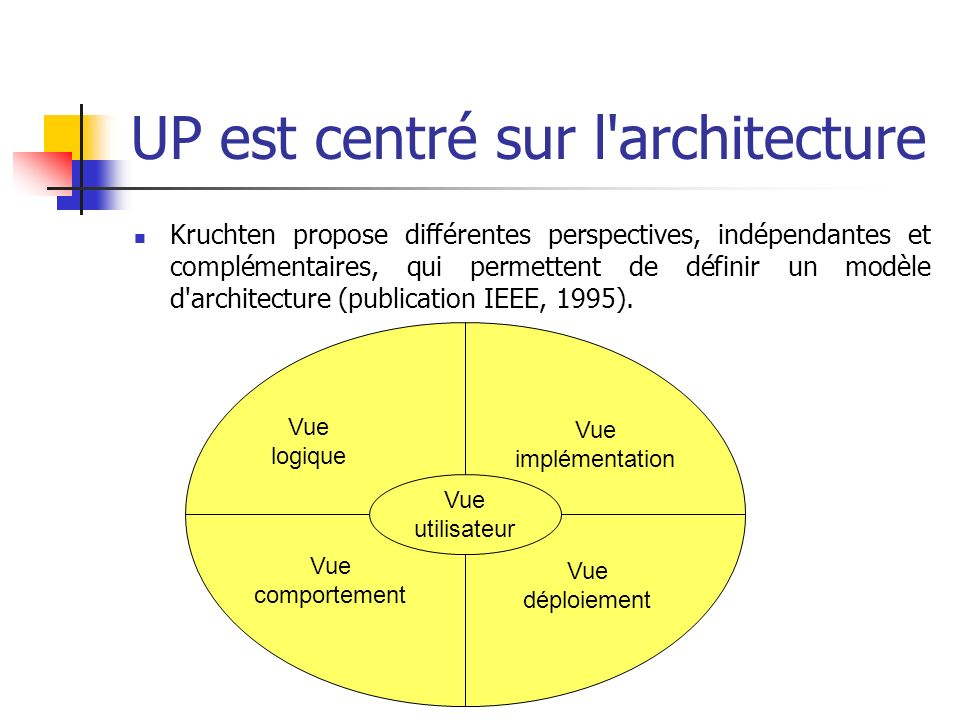
\includegraphics[scale=0.5]{u.jpg}
\caption{ La centralisation du UP sur l'architecture}
\end{center}
\end{figure}



\end{itemize}
\subsubsection{Les phases }
\begin{itemize}[font=\color{black} \Large, label=\ding{74}]
\item \textbf{Analyse des besoins :}
\\
L'analyse des besoins donne une vue du projet sous forme de produit fini. Cette phase porte essentiellement sur les besoins principaux (du point de vue de l'utilisateur), l'architecture générale du système, les risques majeurs, les délais et les coûts. On met en place le projet.

\begin{itemize}[font=\color{black} \Large, label=\ding{73}]
\item Elle répond aux questions suivantes :
\begin{itemize}[font=\color{black} \Large, label=\ding{72}]
\item que va faire le système ? par rapport aux utilisateurs principaux, quels services va-t-il rendre?
\item quelle va être l'architecture générale (cible) de ce système ?
\item quels vont être : les délais, les coûts, les ressources, les moyens à déployer ?
\end{itemize}
\end{itemize}

\end{itemize}
\begin{itemize}[font=\color{black} \Large, label=\ding{74}]
\item \textbf{Elaboration :}
\\

L'élaboration reprend les éléments de la phase d'analyse des besoins et les précise pour arriver à une spécification détaillée de la solution à mettre en œuvre. L'élaboration permet de préciser la plupart des cas d’utilisation, de concevoir l’architecture du système et surtout de déterminer l'architecture de référence. Au terme de cette phase, les chefs de projet doivent être en mesure de prévoir les activités et d’estimer les ressources nécessaires à l’achèvement du projet.
\begin{itemize}[font=\color{black} \Large, label=\ding{73}]
\item Les taches à effectuer dans la phase élaboration sont les suivantes \begin{itemize}[font=\color{black} \Large, label=\ding{72}]
\item Créer une architecture de référence
\item Identifier les risques, ceux qui sont de nature à bouleverser le plan, le coût et le calendrier
\item Définir les niveaux de qualité à atteindre
\item Formuler les cas d'utilisation pour couvrir les besoins fonctionnels et planifier la phase de construction
\item élaborer une offre abordant les questions de calendrier, de personnel et de budget
\end{itemize}
\end{itemize}
\item \textbf{Construction:} 
\begin{flushleft}
La construction est le moment où l’on construit le produit. L’architecture de référence se métamorphose en produit complet. Le produit contient tous les cas d’utilisation que les chefs de projet, en accord avec les utilisateurs ont décidé de mettre au point pour cette version.
\end{flushleft}
\item \textbf{Transition :} 
\begin{flushleft}
Le produit est en version bêta. Un groupe d’utilisateurs essaye le produit et détecte les anomalies et défauts. Cette phase suppose des activités comme la formation des utilisateurs clients, la mise en œuvre d’un service d’assistance et la correction des anomalies constatées.
\end{flushleft}
\end{itemize}
\newpage
\subsubsection{Avantages }
\begin{itemize}[font=\color{green} \Large, label=\ding{52}]

\item Permet de limiter les coûts, en termes de risques, aux strictes dépenses liées à une itération
\item 	Permet de limiter les risques du retard de mise sur le marché du produit développé (identification des problèmes dès les premières states du développement et non en phase de test comme avec l’approche « classique »).
\item Permet d’accélérer le rythme du développement grâce à des objectifs clairs et à court terme.
\item Permet de prendre en compte le fait que les besoins des utilisateurs et les exigences correspondantes ne peuvent être intégralement définies à l’avance et se dégagent peu à peu des itérations successives.  
\end{itemize}
\subsection{Langage de modélisation }
     Dans notre projet, nous utilisons le langage de modélisation graphique à base de pictogrammes en anglais « Unified Modeling Language » (UML). Le langage de modélisation unifié indique précisément quel but était visé lors de la création de ce langage : unifier les langages de modélisation afin que tous puissent utiliser les mêmes concepts. Les concepts propres à UML sont assez génériques que correspondre à une majorité de problématiques.
\\

 Puis, les stéréotypes et les profils permettent de spécialiser le langage pour l’adapter à une problématique particulière. Ainsi, il existe des profils spécifiques pour la modélisation des données. Par contre, il existe sans aucun doute des domaines très particulières où d’autres langages sont bien plus adoptés.
\subsubsection{	Les raisons d’utiliser UML dans nos phases de développement }
\begin{itemize}[font=\color{black} \Large, label=\ding{42}]

\item Pour la modélisation de nos besoins et la conception du système, nous avons choisi d’utiliser le langage UML et ceci pour plusieurs raisons :
\begin{itemize}[font=\color{black} \Large, label=\ding{43}]

	\item UML est un langage normalisé et standardisé par l’OMG (Object Management Group).
	\item UML est un support de communication performant et universel.
	\item UML couvre différentes vues complémentaires d’un système via la définition de plusieurs diagrammes (de l’ordre de 14 pour la version 2.5). Les différents types de diagrammes UML combinés offrent une vue complète des aspects statiques et dynamiques d’un système
\end{itemize}
\end{itemize}
\section*{Conclusion}  
\addcontentsline{toc}{section}{Conclusion}


Ce chapitre a présenté en premier lieu le cadre de mon stage de projet de fin d’études à travers une description générale de l’Institut supérieur d’Informatique et de Gestion Kairouan. En second lieu, il a introduit notre solution proposée par rapport aux attentes de l’institut, et il a présenté les méthodologies et langages choisis pour la modélisation et le suivi du projet. Enfin nous pouvons pencher en détails sur la spécification des besoins. Nous dégageons les besoins fonctionnels et non fonctionnels en élaborant l’étude et la critique de l’existant de l’application. 

\chapter{Phase d’incubation}
\section*{Introduction}  
\addcontentsline{toc}{section}{Introduction} 
La modélisation de notre application est basée sur le formalisme UML. Dans ce chapitre, nous présenterons les objectifs de notre application, ce qui nous amène à identifier les possibilités du système et les besoins des utilisateurs.
\section{Capture des besoins}
\subsection{Description du contexte du système}
\subsubsection{Diagramme de contexte statique}


Le diagramme de contexte statique délimite le domaine d’étude en précisant 
\begin{itemize}[font=\color{black} \Large, label=\ding{88}]

	\item Ce qui est à la charge du système.
	\item En identifiant l’environnement extérieur au système étudié avec lequel ce dernier communique. 
\end{itemize}
\newpage
\begin{itemize}[font=\color{black} \Large, label=\ding{89}]
\item \textbf{Ses composants sont : }
\begin{itemize}[font=\color{black} \Large, label=\ding{90}]
\item Les acteurs externes. Un acteur externe est une entité externe au système étudié qui interagit avec le système. 
\item  Un processus unique symbolisant le Système Information étudié :Nom de SI
\item Echange entre le système étudié et son environnement.
\end{itemize}

\end{itemize}


la figure suivante représenter le diagramme de contexte statique:
\begin{center}
\begin{figure}[h]
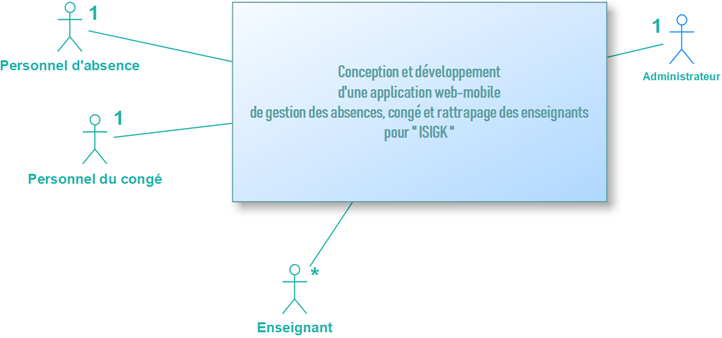
\includegraphics[width= 17 cm ,height= 6cm]{c.png}
\caption{ Diagramme de contexte statique}
\end{figure}
\end{center}
\subsubsection{ Diagramme de contexte dynamique }
Le diagramme de contexte dynamique permet de positionner le système dans son environnement selon le point de vue des communications. Il repend les éléments du contexte statique et précise les échanges des informations qui sont réalisés entre le 
Système et les éléments matériels extérieurs au système. Le système est donc décrit physiquement et logiquement.
\newpage
la figure suivante représenter le diagramme de contexte dynamique:
\begin{figure}[h]
\begin{center}

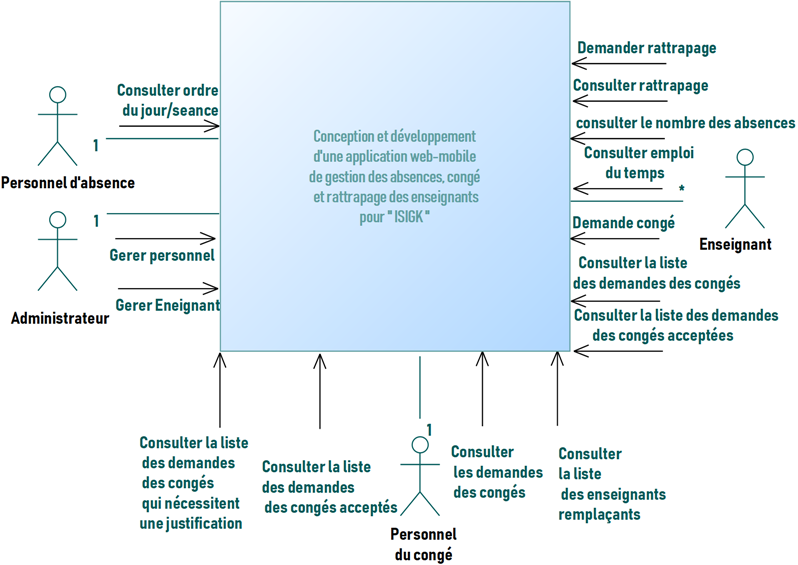
\includegraphics[width= 16 cm ,height= 12 cm]{d.png}
\caption{ Diagramme de contexte Dynamique}
\end{center}

\end{figure}

\subsection{Définition des besoins fonctionnels}
Dans cette partie, nous identifions les acteurs et les différentes fonctionnalités attendues du système. L’application que nous envisageons développer sera exploitée par ces acteurs : Administrateur, Personnel d’absence, Personnel de rattrapage et congé et Enseignant.
\begin{itemize}[font=\color{black} \Large, label=\ding{74}]
\item  	Pour \textbf{l’administrateur}, le système permet de :
\begin{itemize}[font=\color{black} \Large, label=\ding{73}]
\item S’authentifier
\item Gérer les personnels
\item	Gérer les enseignants
\end{itemize}
\newpage
\item  	Pour \textbf{les enseignants}, le système permet de :
\begin{itemize}[font=\color{black} \Large, label=\ding{73}]
\item 	Demander rattrapage
\item consulter la liste des rattrapages
\item 	Demander congé
\item Consulter la liste des congés en cours de traitement
	\item Consulter la liste des demandes des congés traitées
		
		\item consulter l'emploi du temps

\item Consulter le nombre des absences
\end{itemize}




\item Pour\textbf{ le personnel du congé}, le système permet de : 
\begin{itemize}[font=\color{black} \Large, label=\ding{73}]

\item S’authentifier
\item 	Consulter la liste des demandes des congés acceptés
\item 	Consulter la liste des demandes des congés qui nécessitent une justification
\item Consulter les demandes des congés
\item 	Consulter la liste des remplaçants

\end{itemize}
\item  	Pour \textbf{ le personnel d’absence}, le système permet de : 
\begin{itemize}[font=\color{black} \Large, label=\ding{73}]
\item S’authentifier
\item Consulter ordre du jour/séance

\end{itemize}

\end{itemize}

\subsection{Définition des besoins non fonctionnels}
Ce sont les objectifs liés aux performances du système et au contraintes de son environnement. Afin d'avoir un bon fonctionnement de l'application, notre mise en œuvre
doit répondre aux critères suivants :
\begin{itemize}[font=\color{black} \Large, label=\ding{85}] 
\item \textbf{Ergonomie :}\\
les interfaces de notre application doivent être conviviale, simple et aident les utilisateurs à formuler des requêtes correctes.
\item \textbf{	La sécurité  :}\\
Au niveau du contrôle des champs de saisie : notre application doit vérifier la validité des données saisies et en cas d’erreur, il doit afficher un message d’erreur pour que l’utilisateur rectifie les données. Ainsi, il faut s’assurer des cryptages des données au niveau de la base.
\item \textbf{	La fiabilité : }\\les données fournies par l’application doivent être fiables. 
\item \textbf{	La simplicité  :}\\L’application doit présenter des interfaces graphiques simples à manipuler pour tous types d’utilisateurs.
\item \textbf{La disponibilité : }\\
 notre application constitue le cœur de l’activité de l’institut, il est indispensable que cette dernière soit disponible à tout moment.

\end{itemize}

\subsection{Identification des acteurs et des cas d’utilisation}
Nous allons identifier tous les acteurs interagissant avec notre futur système ainsi que l’ensemble
des cas d’utilisations.

\subsubsection{Description détaillée des acteurs}
Le tableau ci-dessous présente une description des acteurs du système:
\begin{table}[htbp]
\begin{center}
\caption{Description détaillée des acteurs \label{table-nom}}
\renewcommand{\arraystretch}{1.8}
\begin{tabular}{|p{5cm}|p{5cm}|p{6cm}|} 
 
\hline 
\cellcolor{PaleTurquoise}\textbf{Acteur} &\cellcolor{PaleTurquoise} \textbf{Définition} &\cellcolor{PaleTurquoise} \textbf{Rôle} \\
\hline
\textbf{Administrateur} & Responsable du bon
déroulement des activités au sein du l'institut.& Supervise les travaux effectués
par les employés et gère les personnels et les enseignants.

 \\
\hline
\textbf{Enseignant}&Renseigne au sein de l'ISIGK&envoie les demandes du congé et de rattrapage et consulte son état d'absence \\
\hline
\textbf{Personnel du congé}& Responsable du bon déroulement de la gestion des congés  des enseignants&  Gère les demandes des congés et ajouter des remplaçants \\
\hline
\textbf{Personnel d'absence}&Responsable du l'état d'absence des enseignants&marque l'état d'absence des enseignants \\
\hline
\end{tabular}
\end{center}
\end{table}
\newpage

\subsubsection{Diagramme du cas d’utilisation général}

la figure  présente les cas d’utilisation réalisés par les utilisateurs du système.
\begin{figure}[h]
 \begin{center}
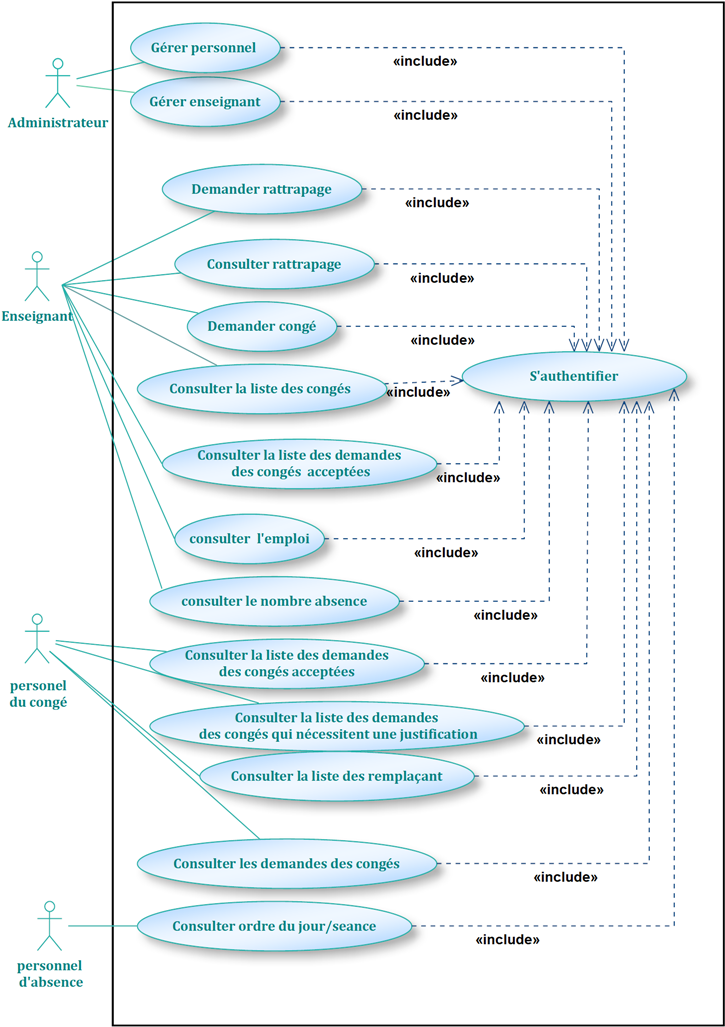
\includegraphics[width= 18 cm ,height= 17 cm]{f.PNG}
\caption{Diagramme du cas d’utilisation général}
\end{center}
\end{figure}
\newpage
\subsection{Raffinement des cas d'utilisation prioritaires}
Dans cette partie, nous avons identifié les acteurs nécessaires de notre application, ainsi que les différents cas d’utilisation relatifs à eux en affectant leurs priorités.
\\ 
le tableau suivant représente l'affectation des acteurs et priorités aux cas d'utilisation:
\begin{table}[htbp]
\begin{center}
\caption{Affectation des acteurs et priorités aux cas d’utilisation \label{table-nom}}
\renewcommand{\arraystretch}{1.7}
\begin{tabular}{|p{5 cm}|p{6 cm}|p{5 cm}|} 
 
\hline 
\cellcolor{PaleTurquoise}\textbf{Acteur} &\cellcolor{PaleTurquoise} \textbf{Cas d’utilisation} &\cellcolor{PaleTurquoise} \textbf{Priorité} \\
\hline
\textbf{Tout les acteurs} & s'authentifier&  1
 \\
\hline
\textbf{Administrateur}&Gérer les personnels& 1 \\
\hline
\textbf{Administrateur}&Gérer les enseignants
& 1 \\
\hline
\textbf{Enseignant}& Demander rattrapage
& 2 \\
\hline
\textbf{Enseignant}& Consulter la liste des rattrapages
& 2 \\
\hline
\textbf{Enseignant}& Demander congé
& 2 \\
\hline
\textbf{Enseignant}& Consulter la liste des congés en cours de traitement
& 2 \\
\hline
\textbf{Enseignant}& Consulter la liste des demandes des congés traitées
& 2 \\
\hline
\textbf{Enseignant}& Consulter l'emploi du temps
& 2 \\
\hline
\textbf{Enseignant}& Consulter la nombre des absences
& 2 \\
\hline

\textbf{Personnel du congé}&   consulter la liste des demandes acceptée & 3 \\
  \hline
\textbf{Personnel du congé}&   Consulter la liste des demandes des congés qui nécessite une justification & 3 \\
\hline
\textbf{Personnel du congé}& Consulter les demandes des congés & 3 \\
 \hline
\textbf{Personnel du congé}&   Consulter la liste des remplaçants & 3 \\
\hline
\textbf{Personnel d'absence}&Consulter l'ordre du jour/séance& 3\\
\hline

\end{tabular}
\end{center}
\end{table}
\newpage
\subsection{Raffinement des cas d’utilisation prioritaires}
À ce niveau de l’activité « Capture des besoins », nous allons raffiner les cas d'utilisation de priorité 1 dont nous allons faire à chacune des cas d'utilisation, la description textuelle de son scénario principal, ainsi que les exceptions qui peuvent se déroulent pendant l'utilisation de l’application.




\subsubsection{Raffinement du cas d'utilisation "S'authentifier"}
la figure suivante représenter le diagramme de cas d’utilisation  relatif à l’acteur \\« Administrateur » qui doit s'authentifier:
\begin{figure}[h]
\begin{center}
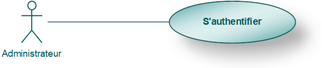
\includegraphics[width= 8cm , height = 1.3cm]{auth.png}
\caption{Description du cas d'utilisation "s'authentifier"}
\end{center}
\end{figure}

l'administrateur doit s'authentifier comme illustre le tableau suivant:
\begin{table}[htbp]
\begin{center}
\caption{Sous Cas d'utilisation "s'authentifier"}
 
 \label{table-nom}
\renewcommand{\arraystretch}{1.6}
\begin{tabular}{|p{17 cm}|}
\hline
\cellcolor{PowderBlue} \textbf{Titre :} S'authentifier \\
 \hline
\cellcolor{MistyRose}  \textbf{Acteur :} Tous les acteurs ( nous allons travailler sur l'exemple du 	l'administrateur)\\
 \hline
 \cellcolor{PowderBlue} \textbf{Résumé :} S'identifier \\
 \hline
 \cellcolor{MistyRose}  \textbf{Pré-condition :} besoin d'accès.\\
 \hline
\cellcolor{PowderBlue} \textbf{Scénario nominal :} 
\begin{itemize}[label=\ding{172}]
\item L’utilisateur demande une connexion au
système 
\end{itemize}
\begin{itemize}[label=\ding{173}]
\item Le Système affiche l’interface de
connexion
\end{itemize}
\begin{itemize}[label=\ding{174}]
\item L’administrateur saisit son login et son
mot de passe
\end{itemize}
\begin{itemize}[label=\ding{175}]
\item Le système vérifie si l’utilisateur existe dans sa base
\end{itemize}
\begin{itemize}[label=\ding{176}]
\item Le système se connecte et ouvre la
session
\end{itemize}
 \\
 \hline
 \cellcolor{MistyRose}  \textbf{Post-condition :} Authentification validée et succès d’accès.\\
 \hline
 \cellcolor{PowderBlue} \textbf{Exception :} Le système affiche un message d’erreur indiquant que le login ou le mot de passe est incorrect. \\
 \hline
\end{tabular}
\end{center}
\end{table}
\newpage
\subsection{Raffinement du cas d’utilisation « Gérer enseignant »}
Ce cas d'utilisation permet à l'administrateur de gérer les enseignants, en ajoutant un enseignant, ou bien en consultant la liste des enseignants comme il peut modifier ou supprimer un enseignant.\\
la figure suivante représente le diagramme du cas d’utilisation  relatif à l’acteur \\« Administrateur » qui a le droit de gérer les enseignants 

 \begin{figure}[h]
 \begin{center}
 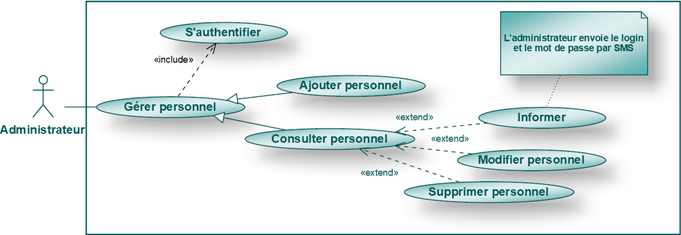
\includegraphics[width= 13 cm ,height= 6 cm]{admin1.png}
\caption{ Diagramme de cas d'utilisation  «Gérer enseignant »}
 \end{center}
\end{figure}


Après être authentifié, l’administrateur peut ajouter un enseignant comme l'illustre le tableau suivant : 
\begin{table}[htbp]
\begin{center}
\caption{Sous Cas d'utilisation "ajouter un enseignant" \label{table-nom}}
\renewcommand{\arraystretch}{1}
\begin{tabular}{|p{17 cm}|}
\hline
\cellcolor{PowderBlue} \textbf{Titre :} Ajouter un enseignant \\
 \hline
\cellcolor{MistyRose}  \textbf{Acteur :} Administrateur\\
 \hline
 \cellcolor{PowderBlue} \textbf{Résumé :} L'administrateur peut ajouter un enseignant \\
 \hline
 \cellcolor{MistyRose}  \textbf{Pré-condition :} S'authentifier.\\
 \hline
\cellcolor{PowderBlue} \textbf{Scénario nominal :} 
\begin{itemize}[label=\ding{172}]
\item L’administrateur demande l’ajout d’un
nouvel enseignant.
\end{itemize}
\begin{itemize}[label=\ding{173}]
\item Le système affiche le formulaire du
nouveau enseignant.
\end{itemize}
\begin{itemize}[label=\ding{174}]
\item L’administrateur remplit le formulaire du
nouveau enseignant et valide l’ajout.
\end{itemize}
\begin{itemize}[label=\ding{175}]
\item Le système vérifie et sauvegarde le
nouveau enseignant.
\end{itemize}

 \\
 \hline
 \cellcolor{MistyRose}  \textbf{Post-condition :} Enseignant ajouté.\\
 \hline
 \cellcolor{PowderBlue} \textbf{Exception :} Dans le cas où l’administrateur entre la matricule du l'enseignant  existant : Le système demande
de vérifier la matricule du nouvel enseignant. \\
 \hline
\end{tabular}
\end{center}
\end{table}
\newpage
la figure suivante représente le diagramme du cas d’utilisation  relatif à l’acteur \\« Administrateur » qui a le droit d'ajouter les enseignants.
\begin{figure}[h]
 \begin{center}
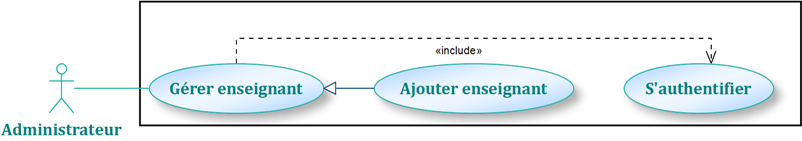
\includegraphics[width= 13 cm ,height= 2cm]{a3.PNG}
\caption{Diagramme du cas d’utilisation "Ajouter enseignant"}
\end{center}
\end{figure}\\
Après être authentifié, l'administrateur peut consulter la liste des enseignants comme l'illustre  tableau suivant : 
\begin{table}[htbp]
\begin{center}
\caption{Sous Cas d'utilisation "Consulter la liste des enseignants" \label{table-nom}}
\renewcommand{\arraystretch}{1}
\begin{tabular}{|p{17 cm}|}
\hline
\cellcolor{PowderBlue} \textbf{Titre :} consulter enseignant \\
 \hline
\cellcolor{MistyRose}  \textbf{Acteur :} Administrateur\\
 \hline
 \cellcolor{PowderBlue} \textbf{Résumé :} L'administrateur peut consulter la liste des enseignants \\
 \hline
 \cellcolor{MistyRose}  \textbf{Pré-condition :} S'authentifier.\\
 \hline
\cellcolor{PowderBlue} \textbf{Scénario nominal :} 
\begin{itemize}[label=\ding{172}]
\item L’administrateur appuis sur le bouton  "consulter la liste des  enseignants".
\end{itemize}
\begin{itemize}[label=\ding{173}]
\item Le système affiche la  liste des enseignants.
\end{itemize}


 \\
 \hline
 \cellcolor{MistyRose}  \textbf{Post-condition :} la liste des enseignants consultée.\\
 \hline
 \cellcolor{PowderBlue}  \textbf{Extensions :}
\begin{itemize} [label=\ding{59}]
\item L’administrateur peut choisir de modifier les informations
d’un enseignant
\item L’administrateur peut choisir de supprimer un enseignant.
\end{itemize} 
   \\
 \hline
\end{tabular}
\end{center}
\end{table}\\
la figure suivante représente le diagramme du cas d’utilisation  relatif à l’acteur \\« Administrateur » qui a le droit de consulter la liste des enseignants.
\begin{figure}[h]
 \begin{center}
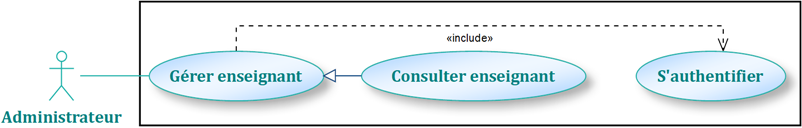
\includegraphics[width=13 cm ,height=2 cm]{a4.PNG}
\caption{Diagramme du cas d’utilisation "consulter enseignant"}
\end{center}
\end{figure}
\newpage
L'administrateur peut modifier un enseignant comme l'illustre le tableau suivant: 
\begin{table}[htbp]
\begin{center}
\caption{Sous Cas d'utilisation "modifier un  enseignant" \label{table-nom}}
\renewcommand{\arraystretch}{1.8}
\begin{tabular}{|p{17 cm}|}
\hline
\cellcolor{PowderBlue} \textbf{Titre :} modifier un enseignant \\
 \hline
\cellcolor{MistyRose}  \textbf{Acteur :} Administrateur\\
 \hline
 \cellcolor{PowderBlue} \textbf{Résumé :} L'administrateur peut modifier un enseignant \\
 \hline
  


 \cellcolor{MistyRose}  \textbf{Pré-condition :} S'authentifier.\\
 \hline
\cellcolor{PowderBlue} \textbf{Scénario nominal :} 
\begin{itemize}[label=\ding{172}]
\item L’administrateur appuis sur le bouton  "consulter la liste des  enseignants".
\end{itemize}
\begin{itemize}[label=\ding{173}]
\item Le système affiche la  liste des enseignants.
\end{itemize}
\begin{itemize}[label=\ding{174}]
\item L’administrateur demande la
modification d’un enseignant.
\end{itemize}
\begin{itemize}[label=\ding{175}]
\item  Le système affiche le formulaire de
enseignant.
\end{itemize}
\begin{itemize}[label=\ding{176}]
\item  L’administrateur modifie les
informations de l'enseignant et valide la
modification.
\end{itemize}
\begin{itemize}[label=\ding{177}]
\item Le système sauvegarde les informations.

\end{itemize}



 \\
 \hline
 \cellcolor{MistyRose}  \textbf{Post-condition :} enseignent modifié.\\
 \hline
 \cellcolor{PowderBlue}  \textbf{Exception :}
Si un champ manque le système affiche un message d’erreur. 
   \\
 \hline
\end{tabular}
\end{center}
\end{table}\\
la figure suivante représente le diagramme du cas d’utilisation  relatif à l’acteur \\« Administrateur » qui a le droit de modifier les informations d'un enseignant.
\begin{figure}[h]
 \begin{center}
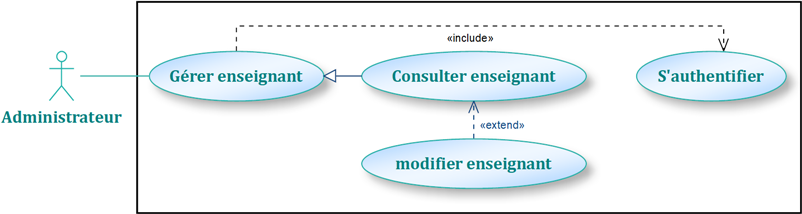
\includegraphics[width=13 cm ,height= 3.8 cm]{a6.PNG}
\caption{Diagramme du cas d’utilisation "modifier enseignant"}
\end{center}
\end{figure}
\newpage
L'administrateur peut supprimer un enseignant comme l’illustre le tableau suivant:
\begin{table}[htbp]
\begin{center}
\caption{Sous Cas d'utilisation "supprimer un  enseignant" \label{table-nom}}
\renewcommand{\arraystretch}{1.9}
\begin{tabular}{|p{17 cm}|}
\hline
\cellcolor{PowderBlue} \textbf{Titre :} Supprimer un enseignant \\
 \hline
\cellcolor{MistyRose}  \textbf{Acteur :} Administrateur\\
 \hline
 \cellcolor{PowderBlue} \textbf{Résumé :} L'administrateur peut supprimer un enseignant \\
 \hline
  


 \cellcolor{MistyRose}  \textbf{Pré-condition :} S'authentifier.\\
 \hline
\cellcolor{PowderBlue} \textbf{Scénario nominal :} 
\begin{itemize}[label=\ding{172}]
\item L’administrateur appuis sur le bouton  "consulter la liste des  enseignants".
\end{itemize}
\begin{itemize}[label=\ding{173}]
\item Le système affiche la  liste des enseignants.
\end{itemize}

\begin{itemize}[label=\ding{174}]
\item L’administrateur sélectionne l’enseignant à
supprimer et demande la suppression.
\end{itemize}
\begin{itemize}[label=\ding{175}]
\item Le système supprime l'enseignant.
\end{itemize}
\begin{itemize}[label=\ding{176}]
\item Le système affiche la validation de
Suppression


\end{itemize}
\\
 \hline
 \cellcolor{MistyRose}  \textbf{Post-condition :} Enseignent supprimé.\\
 \hline
 \cellcolor{PowderBlue}  \textbf{Exception :}
L’administrateur peut annuler la suppression. 
   \\
 \hline
\end{tabular}
\end{center}
\end{table}\\
la figure suivante représente le diagramme du cas d’utilisation  relatif à l’acteur \\« Administrateur » qui a le droit de supprimer un enseignant.
\begin{figure}[h]
 \begin{center}
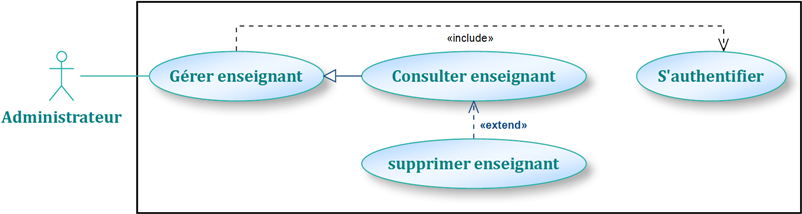
\includegraphics[width=13 cm ,height= 4 cm]{a8.PNG}
\caption{Diagramme du cas d’utilisation "supprimer enseignant"}
\end{center}
\end{figure}


\newpage
L’administrateur doit informer chaque enseignant de son login et son mot de passe comme l'illustre le tableau suivant :
\begin{table}[htbp]

\caption{Sous Cas d'utilisation "Informer" }
\renewcommand{\arraystretch}{1.8}
\begin{tabular}{|p{17 cm}|}
\hline
\cellcolor{PowderBlue} \textbf{Titre :} Informer \\
 \hline
\cellcolor{MistyRose}  \textbf{Acteur :} Administrateur\\
 \hline
 \cellcolor{PowderBlue} \textbf{Résumé :} L'administrateur doit informer chaque enseignant de son login et son mot de passe. \\
 \hline
 \cellcolor{MistyRose}  \textbf{Pré-condition :} 
\begin{itemize}[label=\ding{43}]
\item  S'authentifier.
\item Consulter la liste des enseignants
\end{itemize} 
\\
 \hline
\cellcolor{PowderBlue} \textbf{Scénario nominal :} 
\begin{itemize}[label=\ding{172}]
\item Le système affiche la liste des enseignants.
\end{itemize}
\begin{itemize}[label=\ding{173}]
\item L'administrateur sélectionne un enseignant dans la liste..
\end{itemize}
\begin{itemize}[label=\ding{174}]
\item L'administrateur clique sur le bouton "Informer".
\end{itemize}
\begin{itemize}[label=\ding{175}]
\item Le système affiche une alerte qui signifie que le SMS a été envoyé avec succès
\end{itemize}\\
 \hline
 \cellcolor{MistyRose}  \textbf{Post-condition :} Enseignant informé\\
 \hline
 \cellcolor{PowderBlue} \textbf{Exception :}
Le système affiche un message d'erreur.
  \\
 \hline
\end{tabular}
\end{table} 
\begin{flushleft}
La figure suivante décrit le sous cas d'utilisation "Informer" :
\end{flushleft}
\begin{figure}[h]
\begin{center}
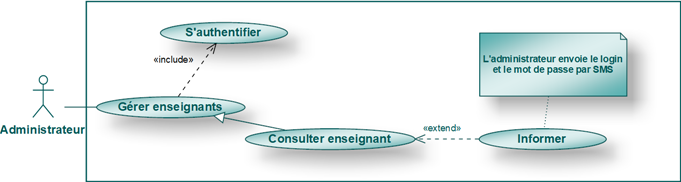
\includegraphics[width= 10cm , height =4cm]{informer_ens.png}
\caption{Sous Cas d'utilisation "Informer"}
\end{center}
\end{figure}
\subsection{Raffinement du cas d’utilisation « Gérer personnel »}
Ce cas d’utilisation permet à l’administrateur de gérer les personnels, en ajoutant
un personnel,ou bien en consultant la liste des personnels dont il peut modifier ou
bien supprimer un personnel.\\
la figure suivante représente le diagramme du cas d’utilisation  relatif à l’acteur \\« Administrateur » qui a le droit de gérer les personnels.
 \begin{figure}[h]
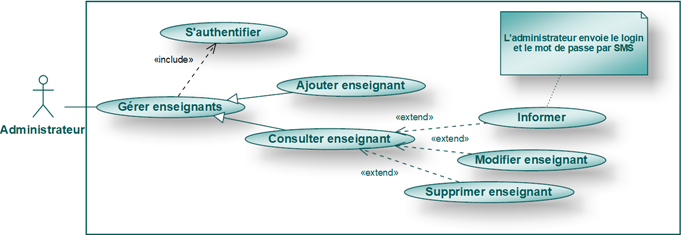
\includegraphics[width= 15 cm ,height= 6 cm]{admin2.png}
\caption{ Diagramme de cas d'utilisation  «Gérer personnel »}
\end{figure}

Après être authentifié, l’administrateur peut ajouter un personnel comme l'illustre le tableau suivant : 
\begin{table}[htbp]
\begin{center}
\caption{Sous Cas d'utilisation "ajouter un personnel" \label{table-nom}}
\renewcommand{\arraystretch}{1}
\begin{tabular}{|p{17 cm}|}
\hline
\cellcolor{PowderBlue} \textbf{Titre :} Ajouter un personnel \\
 \hline
\cellcolor{MistyRose}  \textbf{Acteur :} Administrateur\\
 \hline
 \cellcolor{PowderBlue} \textbf{Résumé :} L'administrateur peut ajouter un personnel \\
 \hline
 \cellcolor{MistyRose}  \textbf{Pré-condition :} S'authentifier.\\
 \hline
\cellcolor{PowderBlue} \textbf{Scénario nominal :} 
\begin{itemize}[label=\ding{172}]
\item L’administrateur demande l’ajout d’un
nouvel personnel.
\end{itemize}
\begin{itemize}[label=\ding{173}]
\item Le système affiche le formulaire du
nouveau personnel.
\end{itemize}
\begin{itemize}[label=\ding{174}]
\item L’administrateur remplit le formulaire du
nouveau personnel  et valide l’ajout.
\end{itemize}
\begin{itemize}[label=\ding{175}]
\item Le système vérifie et sauvegarde le
nouveau personnel.
\end{itemize}

 \\
 \hline
 \cellcolor{MistyRose}  \textbf{Post-condition :} personnel ajouté.\\
 \hline
 \cellcolor{PowderBlue} \textbf{Exception :} Dans le cas où l’administrateur entre une matricule du personnel  existant : Le système demande
de vérifier le matricule du nouvel personnel. \\
 \hline
\end{tabular}
\end{center}
\end{table}\\
la figure suivante représente le diagramme du cas d’utilisation  relatif à l’acteur \\« Administrateur » qui a le droit d'ajouter un enseignant.
\begin{figure}[h]
 \begin{center}
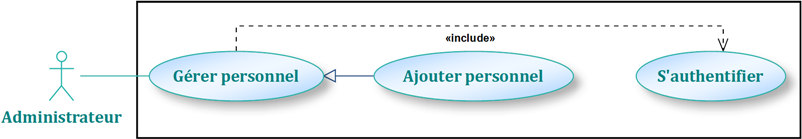
\includegraphics[width=13 cm ,height= 2 cm]{a1.PNG}
\caption{Diagramme du cas d’utilisation "Ajouter personnel"}
\end{center}
\end{figure}



Après être authentifié, l'administrateur peut consulter la liste des personnels comme l'illustre  tableau suivant : 
\begin{table}[htbp]
\begin{center}
\caption{Sous Cas d'utilisation "Consulter la liste des personnels" \label{table-nom}}
\renewcommand{\arraystretch}{1.4}
\begin{tabular}{|p{17 cm}|}
\hline
\cellcolor{PowderBlue} \textbf{Titre :} consulter personnel \\
 \hline
\cellcolor{MistyRose}  \textbf{Acteur :} Administrateur\\
 \hline
 \cellcolor{PowderBlue} \textbf{Résumé :} L'administrateur peut consulter la liste des personnels \\
 \hline
 \cellcolor{MistyRose}  \textbf{Pré-condition :} S'authentifier.\\
 \hline
\cellcolor{PowderBlue} \textbf{Scénario nominal :} 
\begin{itemize}[label=\ding{172}]
\item L’administrateur appuis sur le bouton  "consulter la liste des  personnels".
\end{itemize}
\begin{itemize}[label=\ding{173}]
\item Le système affiche la  liste des personnels.
\end{itemize}


 \\
 \hline
 \cellcolor{MistyRose}  \textbf{Post-condition :} la liste des personnels consultée.\\
 \hline
 \cellcolor{PowderBlue}  \textbf{Extensions :}
\begin{itemize} [label=\ding{59}]
\item L’administrateur peut choisir de modifier les informations
d’un enseignant
\item L’administrateur peut choisir de supprimer un personnel.
\end{itemize} 
   \\
 \hline
\end{tabular}
\end{center}
\end{table}\\
la figure suivante représente le diagramme du cas d’utilisation  relatif à l’acteur \\« Administrateur » qui a le droit de consulter la liste des personnels.
\begin{figure}[h]
 \begin{center}
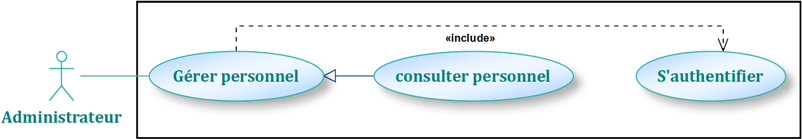
\includegraphics[width=13 cm ,height= 2 cm]{a2.PNG}
\caption{Diagramme du cas d’utilisation "Consulter personnel"}
\end{center}
\end{figure}
\newpage
L'administrateur peut modifier un personnel comme l'illustre le tableau suivant: 
\begin{table}[htbp]
\begin{center}
\caption{Sous Cas d'utilisation "modifier un  personnel" \label{table-nom}}
\renewcommand{\arraystretch}{1.8}
\begin{tabular}{|p{17 cm}|}
\hline
\cellcolor{PowderBlue} \textbf{Titre :} modifier un personnel \\
 \hline
\cellcolor{MistyRose}  \textbf{Acteur :} Administrateur\\
 \hline
 \cellcolor{PowderBlue} \textbf{Résumé :} L'administrateur peut modifier un personnel \\
 \hline
  


 \cellcolor{MistyRose}  \textbf{Pré-condition :} S'authentifier.\\
 \hline
\cellcolor{PowderBlue} \textbf{Scénario nominal :} 
\begin{itemize}[label=\ding{172}]
\item L’administrateur appuis sur le bouton  "consulter la liste des  personnels".
\end{itemize}
\begin{itemize}[label=\ding{173}]
\item Le système affiche la  liste des personnels.
\end{itemize}
\begin{itemize}[label=\ding{174}]
\item L’administrateur demande la
modification d’un personnel.
\end{itemize}
\begin{itemize}[label=\ding{175}]
\item  Le système affiche le formulaire du
personnel.
\end{itemize}
\begin{itemize}[label=\ding{176}]
\item  L’administrateur modifie les
informations du personnel et valide la
modification.
\end{itemize}
\begin{itemize}[label=\ding{177}]
\item Le système sauvegarde les informations.

\end{itemize}



 \\
 \hline
 \cellcolor{MistyRose}  \textbf{Post-condition :} personnel modifié.\\
 \hline
 \cellcolor{PowderBlue}  \textbf{Exception :}
Si un champ manque le système affiche un message d’erreur. 
   \\
 \hline
\end{tabular}
\end{center}
\end{table}\\
la figure suivante représente le diagramme du cas d’utilisation  relatif à l’acteur \\« Administrateur » qui a le droit de modifier les informations d'un personnel:
\begin{figure}[h]
 \begin{center}
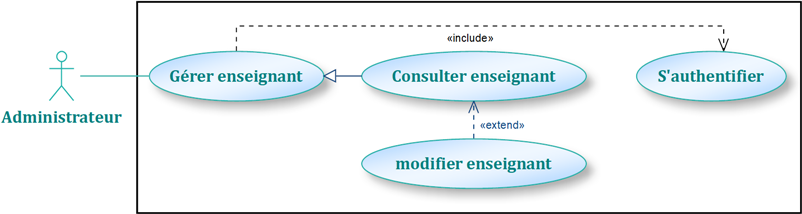
\includegraphics[width=12 cm ,height= 3.5 cm]{a6.PNG}
\caption{Diagramme du cas d’utilisation "Modifier personnel"}
\end{center}
\end{figure}
\newpage
L’administrateur peut supprimer un personnel comme l’illustre le tableau suivant:
\begin{table}[htbp]
\begin{center}
\caption{Sous Cas d'utilisation "supprimer un  personnel" \label{table-nom}}
\renewcommand{\arraystretch}{1.9}
\begin{tabular}{|p{17 cm}|}
\hline
\cellcolor{PowderBlue} \textbf{Titre :} supprimer un personnel \\
 \hline
\cellcolor{MistyRose}  \textbf{Acteur :} Administrateur\\
 \hline
 \cellcolor{PowderBlue} \textbf{Résumé :} L'administrateur peut supprimer un personnel \\
 \hline
  


 \cellcolor{MistyRose}  \textbf{Pré-condition :} S'authentifier.\\
 \hline
\cellcolor{PowderBlue} \textbf{Scénario nominal :} 
\begin{itemize}[label=\ding{172}]
\item L’administrateur appuis sur le bouton  "consulter la liste des  personnels".
\end{itemize}
\begin{itemize}[label=\ding{173}]
\item Le système affiche la  liste des personnels.
\end{itemize}

\begin{itemize}[label=\ding{174}]
\item L’administrateur sélectionne l’enseignant à
supprimer et demande la suppression.
\end{itemize}
\begin{itemize}[label=\ding{175}]
\item Le système supprime le personnel.
\end{itemize}
\begin{itemize}[label=\ding{176}]
\item Le système affiche la validation de
Suppression


\end{itemize}
\\
 \hline
 \cellcolor{MistyRose}  \textbf{Post-condition :} personnel supprimé.\\
 \hline
 \cellcolor{PowderBlue}  \textbf{Exception :}
L’administrateur peut annuler la suppression. 
   \\
 \hline
\end{tabular}
\end{center}
\end{table}\\
la figure suivante représente le diagramme du cas d’utilisation  relatif à l’acteur \\« Administrateur » qui a le droit de supprimer un personnel:
\begin{figure}[h]
 \begin{center}
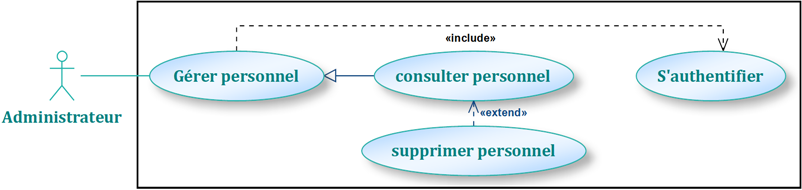
\includegraphics[width=12 cm ,height= 4 cm]{a5.PNG}
\caption{Diagramme du cas d’utilisation "Supprimer personnel"}
\end{center}
\end{figure}
\newpage
L’administrateur doit informer chaque personnel de son login et son mot de passe comme l'illustre le tableau suivant :
\begin{table}[htbp]

\caption{Sous Cas d'utilisation "Informer" }
\renewcommand{\arraystretch}{1.5}
\begin{tabular}{|p{17 cm}|}
\hline
\cellcolor{PowderBlue} \textbf{Titre :} Informer \\
 \hline
\cellcolor{MistyRose}  \textbf{Acteur :} Administrateur\\
 \hline
 \cellcolor{PowderBlue} \textbf{Résumé :} L'administrateur doit informer chaque personnel de son login et son mot de passe. \\
 \hline
 \cellcolor{MistyRose}  \textbf{Pré-condition :} 
\begin{itemize}[label=\ding{43}]
\item  S'authentifier.
\item Consulter la liste des personnels
\end{itemize} 
\\
 \hline
\cellcolor{PowderBlue} \textbf{Scénario nominal :} 
\begin{itemize}[label=\ding{172}]
\item Le système affiche la liste des personnels.
\end{itemize}
\begin{itemize}[label=\ding{173}]
\item L'administrateur sélectionne un personnel dans la liste.
\end{itemize}
\begin{itemize}[label=\ding{174}]
\item L'administrateur clique sur le bouton "Informer".
\end{itemize}
\begin{itemize}[label=\ding{175}]
\item Le système affiche une alerte qui signifie que le SMS a été envoyé avec succès
\end{itemize}\\
 \hline
 \cellcolor{MistyRose}  \textbf{Post-condition :} Personnel informé\\
 \hline
 \cellcolor{PowderBlue} \textbf{Exception :}
Le système affiche un message d'erreur.
  \\
 \hline
\end{tabular}
\end{table} 
\begin{flushleft}
La figure suivante décrit le sous cas d'utilisation "Informer" :
\end{flushleft}
\begin{figure}[h]
\begin{center}
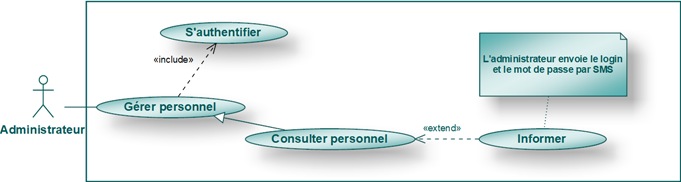
\includegraphics[width= 10cm , height =4cm]{informer_per.png}
\caption{Sous Cas d'utilisation "Informer"}
\end{center}
\end{figure}
\newpage
\section{Analyse des cas d’utilisation prioritaires }
Le modèle d’analyse doit fournir une approche conceptuelle du problème. Ce modèle a
pour but de définir une structure robuste et extensible qui nous servira de base pour la
construction du système.
Le modèle d’analyse doit aussi fournir des spécifications fonctionnelles totales du système
que l’on veut développer sans aucune référence à l’environnement de développement. La
phase de développement (conception et implémentation) sera conduite à partir de ce
modèle.
L’analyse d’un cas d’utilisation consiste à représenter : les diagrammes de traçabilité et les
diagrammes de collaboration.

\subsection{Traçabilité entre le modèle du cas d’utilisation (MCU) et le modèle d’analyse (MA)}
\begin{itemize}[font=\color{black} \Large, label=\ding{70}]
\item À ce niveau de l’activité « Analyse » de la phase d’incubation, nous avons précis les tables relatives aux cas d’utilisation ainsi que les interfaces utilisateurs et les contrôles de chaque cas d’utilisation.
\item \textbf{ Diagramme de traçabilité} : Ce modèle représente les différentes interfaces,
commandes et entités impliqués dans l'exécution d'un cas d'utilisation, il permet le
passage du modèle à utiliser l'analyse de cas d’utilisation.


 Dans ce
dernier, trois classes d’analyse y participent :
\begin{itemize}[font=\color{black} \Large, label=\ding{71}]
\item \textbf{Une classe « interface »:}
 qui permet à
l’acteur d’interagir avec le
système. 
l’utilisateur.

\begin{figure}[h]
 \begin{center}

\includegraphics[width= 1 cm ,height= 1 cm]{int.png}
\caption{ classe « interface »}
\end{center}
\end{figure}


\item \textbf{Une Classe « Contrôle »:}
qui gère le contrôle des données
et la coordination des autres
classes. Elle représente les informations persistantes
\begin{figure}[h]
 \begin{center}

\includegraphics[width= 1cm ,height= 1 cm]{cntrl.png}
\caption{ classe « interface »}
\end{center}
\end{figure}

\item \textbf{Des Classes « entités »:}
qui
représentent les sources
d’informations à partir
desquels nous allons extraire
les données . Elles contiennent
des opérations dans le but d’entrer et stocker
l’information et de créer et
supprimer les objets de la
classe.
\end{itemize}
\begin{figure}[h]
 \begin{center}

\includegraphics[width= 1 cm ,height= 1 cm]{entite.png}
\caption{ Classe « entité »}
\end{center}
\end{figure}

\end{itemize}

\subsubsection{Traçabilité entre MCU et MA relatif au cas d’utilisation "S’authentifier" }
La figure  montre la traçabilité entre le modèle de cas d’utilisation «s'authentifier » et le modèle
d’analyse:

\begin{figure}[h]
\begin{center}
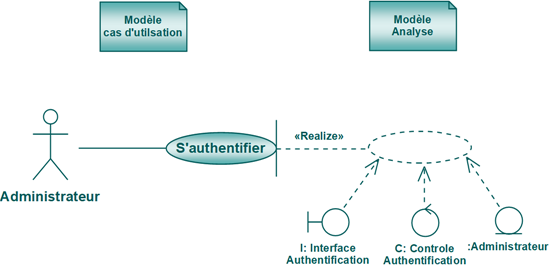
\includegraphics[width= 14cm , height =8cm]{t1.png}
\caption{Traçabilité entre MCU et MA relatif au cas d’utilisation "S’authentifier"}
\end{center}
\end{figure} 
\newpage
\subsubsection{Traçabilité entre MCU et MA relatif au cas d’utilisation "Ajouter enseignant" }
La figure  montre la traçabilité entre le modèle de cas d’utilisation « Ajouter enseignant » et le modèle
d’analyse:

\begin{figure}[h]
\begin{center}
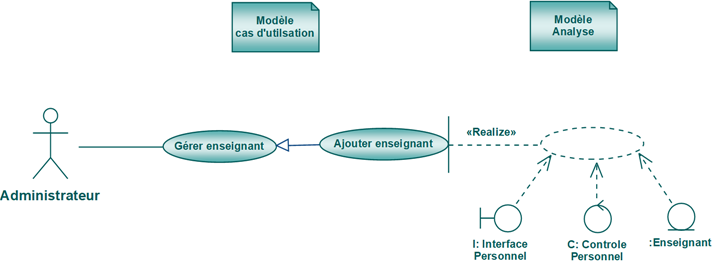
\includegraphics[width= 14cm , height =5.5cm]{aj_ens.png}
\caption{Traçabilité entre MCU et MA relatif au cas d’utilisation "Ajouter enseignant"}
\end{center}
\end{figure}
\subsubsection{Traçabilité entre MCU et MA relatif au cas d’utilisation "consulter la liste des enseignants" }
La figure  montre la traçabilité entre le modèle de cas d’utilisation «consulter la liste des enseignant » et le modèle
d’analyse:
\begin{figure}[h]
\begin{center}
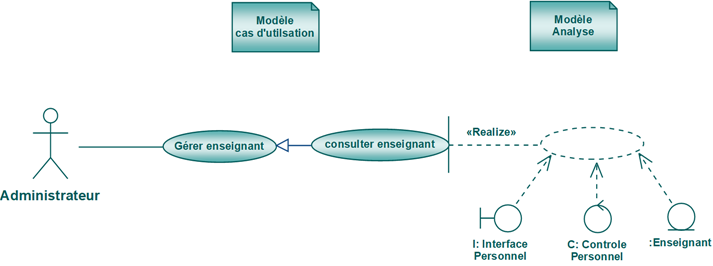
\includegraphics[width= 13cm , height =6cm]{traconsens.png}
\caption{Traçabilité entre MCU et MA relatif au cas d’utilisation "consulter la liste des enseignants"}
\end{center}
\end{figure} 



\subsubsection{Traçabilité entre MCU et MA relatif au cas d’utilisation "Modifier un enseignant" }
La figure  montre la traçabilité entre le modèle de cas d’utilisation «modifier un enseignant » et le modèle
d’analyse:
\begin{figure}[h]
\begin{center}
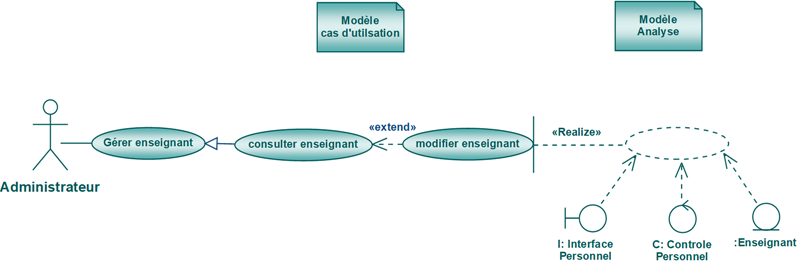
\includegraphics[width= 13cm , height =6cm]{mod_ens.png}
\caption{Traçabilité entre MCU et MA relatif au cas d’utilisation "Modifier un enseignant"}
\end{center}
\end{figure} 
\subsubsection{Traçabilité entre MCU et MA relatif au cas d’utilisation "Supprimer un enseignant" }
La figure  montre la traçabilité entre le modèle de cas d’utilisation «supprimer un enseignant » et le modèle
d’analyse:
\begin{figure}[h]
\begin{center}
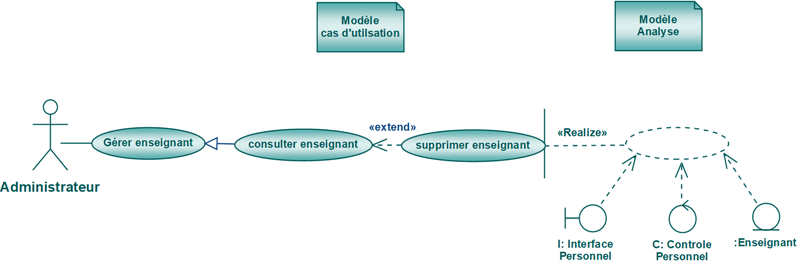
\includegraphics[width= 13cm , height =5cm]{sup_ens.png}
\caption{Traçabilité entre MCU et MA relatif au cas d’utilisation "Supprimer un enseignant"}
\end{center}
\end{figure} 
\subsubsection{Traçabilité entre MCU et MA relatif au cas d’utilisation "Informer enseignant" }
\begin{figure}[h]
\begin{center}
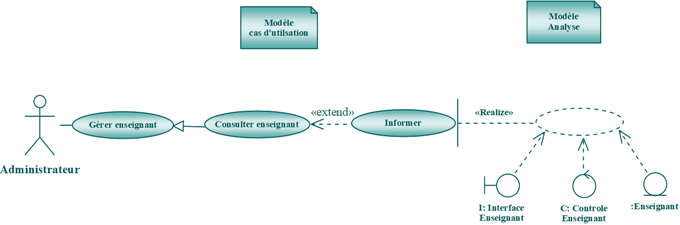
\includegraphics[width= 13cm , height =5cm]{tra_info_ens.png}
\caption{Traçabilité entre MCU et MA relatif au cas d’utilisation "Informer enseignant"}
\end{center}
\end{figure}
\subsubsection{Traçabilité entre MCU et MA relatif au cas d’utilisation "Ajouter personnel" }
La figure  montre la traçabilité entre le modèle de cas d’utilisation « Ajouter personnel » et le modèle
d’analyse:
\begin{figure}[h]
\begin{center}
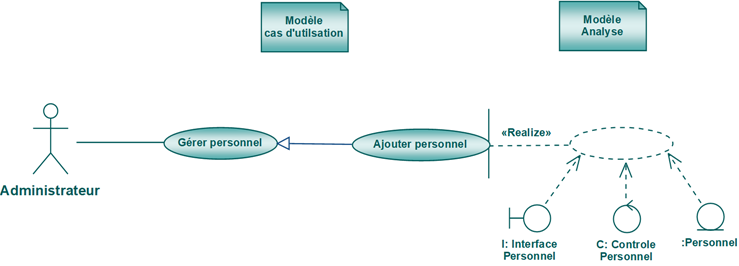
\includegraphics[width= 14cm , height =6cm]{tap.png}
\caption{Traçabilité entre MCU et MA relatif au cas d’utilisation "Ajouter personnel"}
\end{center}
\end{figure}
\subsubsection{Traçabilité entre MCU et MA relatif au cas d’utilisation "consulter la liste des personnels" }
La figure  montre la traçabilité entre le modèle de cas d’utilisation « consulter la liste des personnels » et le modèle
d’analyse:
\begin{figure}[h]
\begin{center}
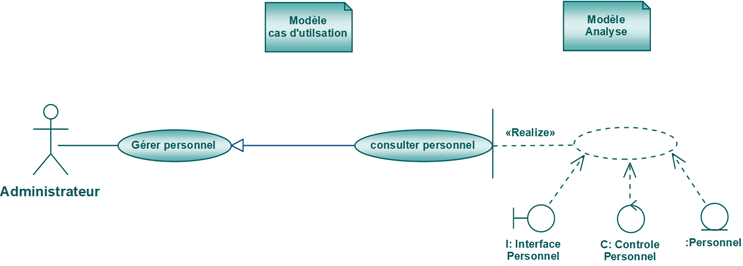
\includegraphics[width= 14cm , height =6cm]{traconsabs.png}
\caption{Traçabilité entre MCU et MA relatif au cas d’utilisation "consulter la liste des personnels"}
\end{center}
\end{figure} 


\subsubsection{Traçabilité entre MCU et MA relatif au cas d’utilisation "Modifier un personnel" }
La figure  montre la traçabilité entre le modèle de cas d’utilisation « Modifier un personnel» et le modèle
d’analyse:
\begin{figure}[h]
\begin{center}
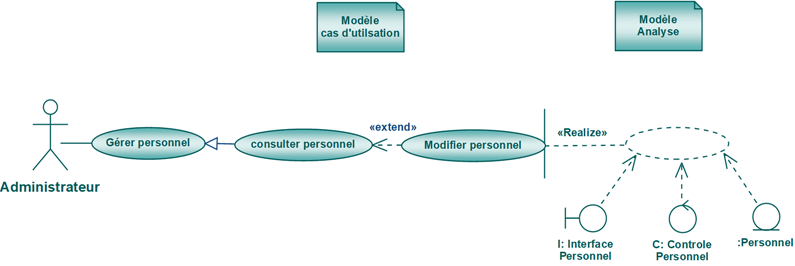
\includegraphics[width= 14cm , height =5cm]{tma.png}
\caption{Traçabilité entre MCU et MA relatif au cas d’utilisation "Modifier un personnel"}
\end{center}
\end{figure}

\subsubsection{Traçabilité entre MCU et MA relatif au cas d’utilisation "Supprimer un personnel" }
La figure  montre la traçabilité entre le modèle de cas d’utilisation « Supprimer un personnel» et le modèle
d’analyse:
\begin{figure}[h]
\begin{center}
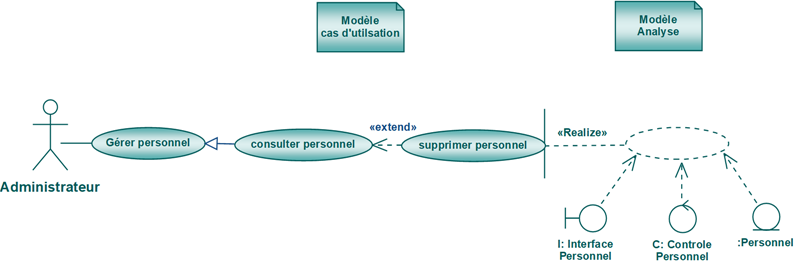
\includegraphics[width= 14cm , height =6cm]{tracsupp.png}
\caption{Traçabilité entre MCU et MA relatif au cas d’utilisation "Supprimer un personnel" }
\end{center}
\end{figure} 
\subsubsection{Traçabilité entre MCU et MA relatif au cas d’utilisation "Informer personnel" }
\begin{figure}[h]
\begin{center}
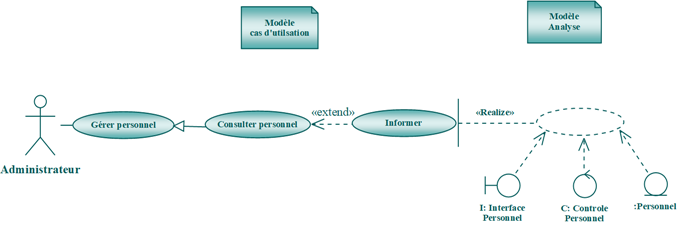
\includegraphics[width= 14cm , height =6cm]{tra_info_per.png}
\caption{Traçabilité entre MCU et MA relatif au cas d’utilisation "Informer personnel"}
\end{center}
\end{figure}
\newpage
\subsection{Diagrammes de classes d'analyse}
\begin{itemize}[font=\color{black} \Large, label=\ding{70}] 
\item À ce niveau de l’activité « Analyse » de la phase d’incubation, nous allons présenter les relations entre les tables, les acteurs, les contrôles et les interfaces de quelques cas d‘utilisation.
\end{itemize}
\subsubsection{Diagramme de classes d’analyse relatif au cas d’utilisation "S’authentifier" }
La figure  représente les relations entre la table utilisée « Administrateur » dans le cas d’utilisation « s'authentifier », l’interface  authentification et  l'entité de  contrôle d'authentification:
\begin{figure}[h]
\begin{center}

\includegraphics[width= 12cm , height =2cm]{classid.png}
\caption{Diagramme de classes d’analyse relatif au cas d’utilisation "S’authentifier"}
\end{center}
\end{figure}
\subsubsection{Diagramme de classes d’analyse relatif au cas d’utilisation "Gérer enseignant" }
La figure  représente les relations entre la table utilisée « Enseignant » dans le cas d’utilisation « Gérer enseignant », l’interface d'un enseignant et  l'entité de  contrôle d'un enseignant:
\begin{figure}[h]
\begin{center}
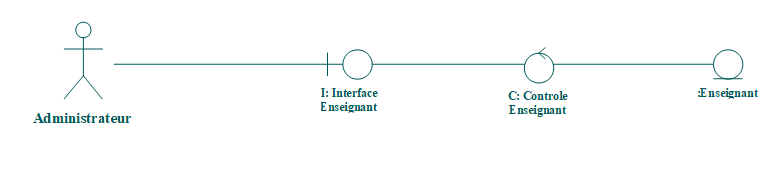
\includegraphics[width= 12cm , height =3.6cm]{cl_aj.png}
\caption{Diagramme de classes d’analyse relatif au cas d’utilisation "Gérer enseignant"}
\end{center}
\end{figure}
\subsubsection{Diagramme de classes d’analyse relatif au cas d’utilisation "Gérer personnel" }
La figure  représente les relations entre la table utilisée « Personnel » dans le cas d’utilisation « Gérer personnel », l’interface d'un personnel et  l'entité de  contrôle d'un personnel:
\begin{figure}[h]
\begin{center}
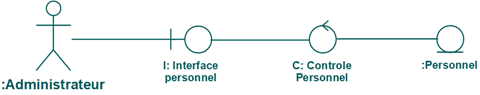
\includegraphics[width= 12cm , height =2cm]{cap.png}
\caption{Diagramme de classes d’analyse relatif au cas d’utilisation "Gérer personnel"}
\end{center}
\end{figure}
\subsection{Diagrammes de collaboration }

\begin{itemize}[font=\color{black} \Large, label=\ding{70}]
\item À ce niveau de l’activité « Analyse » de la phase d’incubation, nous allons élaborer les diagrammes de collaboration des cas des utilisations prioritaires, qui permet de décrire les interactions entre les
objets intervenant dans la réalisation d’un scénario d’un cas d’utilisation.
\item  \textbf{Diagramme de collaboration :} est un diagramme d’interaction organisée entre les
rôles qui interagissent et les liens qui les assemblent. Il montre les relations entre les objets jouant les différents rôles. Toutefois, un diagramme de collaboration ne doit contenir aucune notion de temps. Contenu : Échange de messages, au niveau du contexte :
acteurs, objets ou états, liens, messages, itération, contrainte.
\end{itemize}
\newpage
\subsubsection{Diagramme de collaboration relatif au cas d’utilisation "S’authentifier" }
La figure suivante présente un diagramme de collaboration qui décrit les différents
scénarios possibles pour le cas "S'authentifier"
\begin{figure}[h]
\begin{center}
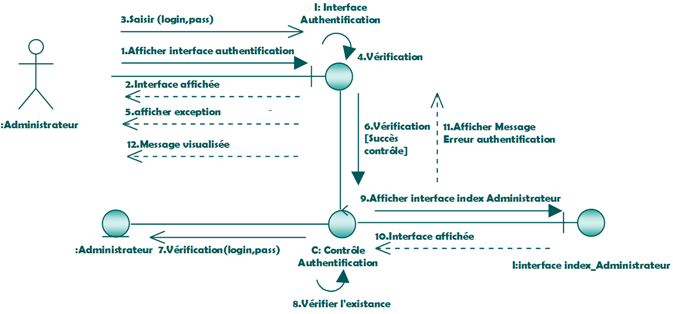
\includegraphics[width= 14cm , height =5.5cm]{colla_adm_authentification.png}
\caption{Diagramme de collaboration relatif au cas d’utilisation «S’authentifier»}
\end{center}
\end{figure}

\subsubsection{Diagramme  de  collaboration  de  modèle  d'analyse  pour  le  cas  d'utilisation «Ajouter enseignant»  }
La figure suivante présente un diagramme de collaboration qui décrit les différents
scénarios possibles pour le cas "Ajouter enseignant"
\begin{figure}[h]
\begin{center}
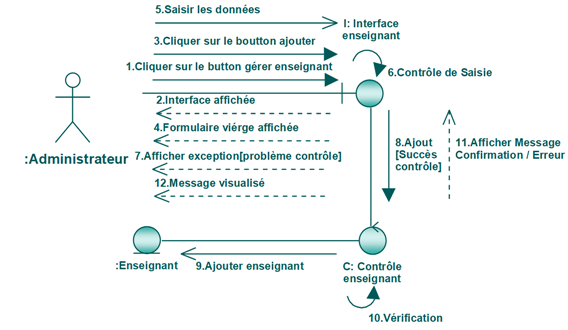
\includegraphics[width= 14 cm , height =5.5 cm]{collaajoutens.png}
 \caption{Diagramme  de  collaboration  de  modèle  d'analyse  pour  le  cas  d'utilisation «Ajouter enseignant»}
\end{center}
\end{figure}
\subsubsection{Diagramme de collaboration pour le modèle d’analyse du cas d'utilisation                                       «Consulter enseignant»}
La figure suivante présente un diagramme de collaboration qui décrit les différents
scénarios possibles pour le cas "consulter enseignant"
\begin{figure}[h]
 \begin{center}
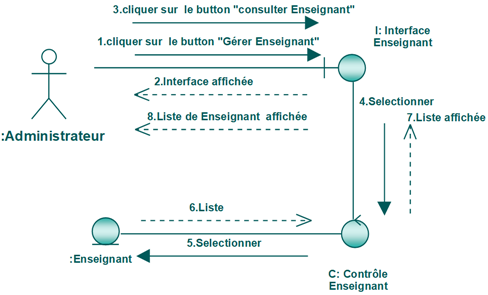
\includegraphics[width= 14 cm ,height=5.5cm]{collaconsens.PNG}
\caption{Diagramme de collaboration pour le modèle d’analyse du cas d'utilisation                                       «Consulter enseignant»}

\end{center}
\end{figure}

\subsubsection{Diagramme  de  collaboration  de  modèle  d'analyse  pour  le  cas  d'utilisation «Modifier enseignant»  }
La figure suivante présente un diagramme de collaboration qui décrit les différents
scénarios possibles pour le cas "Modifier enseignant"
\begin{figure}[h]
\begin{center}
\includegraphics[width= 14 cm , height =6 cm]{colla_adm_modifierenseignant.png}
 \caption{Diagramme  de  collaboration  de  modèle  d'analyse  pour  le  cas  d'utilisation «Modifier enseignant»}
\end{center}
\end{figure}
\subsubsection{Diagramme  de  collaboration  de  modèle  d'analyse  pour  le  cas  d'utilisation "Supprimer enseignant"  }
La figure suivante présente un diagramme de collaboration qui décrit les différents
scénarios possibles pour le cas "Supprimer enseignant":
\begin{figure}[h]
\begin{center}
\includegraphics[width= 12 cm , height =6cm]{colla_adm_supprimerenseignant.png}
 \caption{Diagramme  de  collaboration  de  modèle  d'analyse  pour  le  cas  d'utilisation «Supprimer enseignant» }
\end{center}
\end{figure}
\subsubsection{Diagramme  de  collaboration  de  modèle  d'analyse  pour  le  cas  d'utilisation «Informer personnel»  }
La figure suivante présente un diagramme de collaboration qui décrit les différents
scénarios possibles pour le cas "Informer personnel":
\begin{figure}[h]
\begin{center}
\includegraphics[width= 12 cm , height =7 cm]{colla_admin_informerpersonnel.png}
 \caption{Diagramme  de  collaboration  de  modèle  d'analyse  pour  le  cas  d'utilisation "Informer personnel"}
\end{center}
\end{figure}
\subsubsection{Diagramme de collaboration pour le modèle d’analyse du cas d'utilisation                                       «Ajouter personnel»}
La figure suivante présente un diagramme de collaboration qui décrit les différents
scénarios possibles pour le cas "Ajouter personnel":\begin{figure}[h]
 \begin{center}
\includegraphics[width= 12 cm ,height=  5.5cm]{collaajoutper.PNG}
\caption{Diagramme de collaboration pour le modèle d’analyse du cas d'utilisation                                       «Ajouter personnel»}

\end{center}
\end{figure}
\subsubsection{Diagramme de collaboration pour le modèle d’analyse du cas d'utilisation                                       «Consulter personnel»}
La figure suivante présente un diagramme de collaboration qui décrit les différents
scénarios possibles pour le cas "Consulter personnel":
\begin{figure}[h]
 \begin{center}
\includegraphics[width= 14 cm ,height=  5cm]{collaconsper.PNG}
\caption{Diagramme de collaboration pour le modèle d’analyse du cas d'utilisation                                       «Consulter personnel»}

\end{center}
\end{figure}
\subsubsection{Diagramme de collaboration pour le modèle d’analyse du cas d'utilisation                                       «Modifier personnel»}
La figure suivante présente un diagramme de collaboration qui décrit les différents
scénarios possibles pour le cas "Modifier personnel":
\begin{figure}[h]
 \begin{center}
\includegraphics[width= 14 cm ,height=  6.5cm]{colla_adm_modifierpersonnel.PNG}
\caption{Diagramme de collaboration pour le modèle d’analyse du cas d'utilisation                                       «Modifier personnel»}

\end{center}
\end{figure}
\subsubsection{Diagramme de collaboration pour le modèle d’analyse du cas d'utilisation                                       «Supprimer personnel»}
La figure suivante présente un diagramme de collaboration qui décrit les différents
scénarios possibles pour le cas "Supprimer personnel":
\begin{figure}[h]
 \begin{center}
\includegraphics[width= 12 cm ,height=  7cm]{colla_adm_supprimerpersonnel.PNG}
\caption{Diagramme de collaboration pour le modèle d’analyse du cas d'utilisation                                       «Supprimer personnel»}

\end{center}
\end{figure}
\subsubsection{Diagramme  de  collaboration  de  modèle  d'analyse  pour  le  cas  d'utilisation «Informer personnel»  }
La figure suivante présente un diagramme de collaboration qui décrit les différents
scénarios possibles pour le cas "Informer personnel":
\begin{figure}[h]
\begin{center}
\section{Conception des cas d’utilisation prioritaires :}
La conception dans cette phase consiste à concevoir les cas d’utilisations, nous allons construire alors les diagrammes de classes de conception, ainsi que les interactions entre eux et les diagrammes de séquence de chaque cas d’utilisation de priorité 1.
\subsection{Diagrammes des classes de conception :}
le diagramme de classes exprime l'aspect statistique du système en termes de classes et de relations entre ces classes.Il nous permet de présenter la structure interne du système et d'organiser le travail de développeur .
\subsubsection{Diagramme de classes de conception relatif au cas d’utilisation «S’authentifier» :}
La figure  représente les classes du cas d’utilisation « S’authentifier » et les relations entre elles.
\begin{figure}[h]
 \begin{center}
\includegraphics[width= 12 cm ,height=  3.5cm]{cl_auth.PNG}
\caption{Diagramme de classes de conception relatif au cas d’utilisation «S’authentifier» }

\end{center}
\end{figure}
\subsubsection{Diagramme de classes de conception relatif au cas d’utilisation «Gérer enseignant» :}
La figure  représente les classes du cas d’utilisation « Gérer enseignant » et les relations entre elles.
\begin{figure}[h]
 \begin{center}
\includegraphics[width= 11 cm ,height= 5cm]{cl_ge.PNG}
\caption{Diagramme de classes de conception relatif au cas d’utilisation «Gérer enseignant»}

\end{center}
\end{figure}

\subsubsection{Diagramme de classes de conception relatif au cas d’utilisation «Gérer personnel» :}
La figure  représente les classes du cas d’utilisation « Gérer personnel » et les relations entre elles.
\begin{figure}[h]
 \begin{center}
\includegraphics[width= 11 cm ,height=  7cm]{cl_gp.PNG}
\caption{Diagramme de classes de conception relatif au cas d’utilisation «Gérer personnel» }

\end{center}
\end{figure}



\subsection{Diagrammes de séquences :}
Dans cette partie de conception nous allons utiliser le diagramme de séquence pour modéliser les fonctionnements des cas d'utilisation.les diagramme de séquence mettent en valeur les échanges de message(déclenchant des événements)entre acteurs et objets ou entre objets et objets de manière chronologique(facture de temps),l'évolution du temps se lit de haut en bas.
\newpage
\subsubsection{Diagramme de séquences relatif au cas d’utilisation « S’authentifier » :}
la figure   présente un diagramme de séquence qui illustre une description détaillée du scénario relatif au cas d’utilisation « S’authentifier »: 
{\begin{figure}[h]
 \begin{center}
\includegraphics[width= 18 cm ,height=  17cm]{ca.PNG}
\caption{Diagramme de séquences relatif au cas d’utilisation « S’authentifier »}

\end{center}
\end{figure}}
\newpage
\subsubsection{Diagramme de séquences relatif au cas d’utilisation « Ajouter enseignant » :}
la figure   présente un diagramme de séquence qui illustre une description détaillée du scénario relatif au cas d’utilisation « Ajouter enseignant»: 
{\begin{figure}[h]
 \begin{center}
\includegraphics[width= 18 cm ,height=  17cm]{sae.PNG}
\caption{Diagramme de séquences relatif au cas d’utilisation « Ajouter enseignant »}

\end{center}
\end{figure}}
\newpage
\subsubsection{Diagramme de séquences relatif au cas d’utilisation « Consulter enseignant » :}
la figure   présente un diagramme de séquence qui illustre une description détaillée du scénario relatif au cas d’utilisation «  Consulter enseignant»: 
{\begin{figure}[h]
 \begin{center}
\includegraphics[width= 18 cm ,height=  17cm]{sec_cons_ens.PNG}
\caption{Diagramme de séquences relatif au cas d’utilisation « Consulter enseignant »}

\end{center}
\end{figure}}
\newpage
\subsubsection{Diagramme de séquences relatif au cas d’utilisation « Modifier enseignant » :}
la figure   présente un diagramme de séquence qui illustre une description détaillée du scénario relatif au cas d’utilisation «  Modifier enseignant»: 
{\begin{figure}[h]
 \begin{center}
\includegraphics[width= 18 cm ,height= 17cm]{sec_modif_ens.PNG}
\caption{Diagramme de séquences relatif au cas d’utilisation « Modifier enseignant »}

\end{center}
\end{figure}}
\newpage
\subsubsection{Diagramme de séquences relatif au cas d’utilisation « Supprimer enseignant » :}
la figure   présente un diagramme de séquence qui illustre une description détaillée du scénario relatif au cas d’utilisation «  Supprimer enseignant»: 
{\begin{figure}[h]
 \begin{center}
\includegraphics[width= 18cm ,height=  17cm]{sec_sup_ens.PNG}
\caption{Diagramme de séquences relatif au cas d’utilisation « Supprimer enseignant »}

\end{center}
\end{figure}}
\newpage
\subsubsection{Diagramme de séquences relatif au cas d’utilisation « Ajouter personnel » :}
la figure   présente un diagramme de séquence qui illustre une description détaillée du scénario relatif au cas d’utilisation «  Ajouter personnel »: 
{\begin{figure}[h]
 \begin{center}
\includegraphics[width= 14 cm ,height=  12cm]{sap.PNG}
\caption{Diagramme de séquences relatif au cas d’utilisation « Ajouter personnel  »}

\end{center}
\end{figure}}
\newpage
\subsubsection{Diagramme de séquences relatif au cas d’utilisation « Consulter personnel » :}
la figure   présente un diagramme de séquence qui illustre une description détaillée du scénario relatif au cas d’utilisation « Consulter personnel »: 
{\begin{figure}[h]
 \begin{center}
\includegraphics[width= 18 cm ,height=  17cm]{sec_cons_per.PNG}
\caption{Diagramme de séquences relatif au cas d’utilisation « Consulter personnel  »}

\end{center}
\end{figure}}
\newpage
\subsubsection{Diagramme de séquences relatif au cas d’utilisation « Modifier personnel » :}
la figure   présente un diagramme de séquence qui illustre une description détaillée du scénario relatif au cas d’utilisation « Modifier personnel »: 
{\begin{figure}[h]
 \begin{center}
\includegraphics[width= 18 cm ,height=  17cm]{sec_modif_per.PNG}
\caption{Diagramme de séquences relatif au cas d’utilisation « Modifier personnel  »}

\end{center}
\end{figure}}
\newpage
\subsubsection{Diagramme de séquences relatif au cas d’utilisation « Supprimer personnel » :}
la figure   présente un diagramme de séquence qui illustre une description détaillée du scénario relatif au cas d’utilisation « Supprimer personnel »: 
{\begin{figure}[h]
 \begin{center}
\includegraphics[width= 18 cm ,height=  17cm]{sec_sup_per.PNG}
\caption{Diagramme de séquences relatif au cas d’utilisation « Supprimer personnel  »}

\end{center}
\end{figure}}
\newpage
\section{Implémentation}
\subsection{Environnement de développement}

Dans cette partie , nous allons identifier notre environnement du développement matériel et logiciel.
\begin{itemize}[font=\color{black} \Large, label=\ding{105}] 
\item \textbf{Système d'exploitation :} windows 10 .
\item \textbf{Machine :} HP i5-3210M CPU @ 2.50GHz .
\item \textbf{Outil de rédaction :} Latex .
\item \textbf{Outil de modélisation :} Pacestar UML Diagrammer .
\item \textbf{Outil de développement:} 
\begin{gitemize}
\item \textbf{Brackets :} \newline
 Brackets est un éditeur open source pour le web design et le développement sur des technologies Web telles que HTML, CSS et JavaScript. Le projet a été créé et est maintenu par Adobe, et est publié sous une licence MIT. 
 \end{gitemize}
 \begin{fitemize}
  \item \textbf{Visual Studio Code :}\\ est présenté lors de la conférence des développeurs Build d'avril 2015 comme un éditeur de code cross-platform, open source et gratuit, supportant une dizaine de langages
Le code source est fourni sous la licence libre MIT (plus précisément la licence Expat) sur le site du projet sur Github. En revanche, l'exécutable est proposé sur le site officiel de Microsoft sous une licence privatrice.
 \end{fitemize}
 \begin{hitemize}
 \item \textbf{XAMPP :} \\
 XAMPP est un ensemble de logiciels permettant de mettre en place facilement un serveur Web local, un serveur FTP et un serveur de messagerie électronique. Il s'agit d'une distribution de logiciels libres (X (cross) Apache MariaDB Perl PHP) offrant une bonne souplesse d'utilisation, réputée pour son installation simple et rapide. Ainsi, il est à la portée d'un grand nombre de personnes puisqu'il ne requiert pas de connaissances particulières et fonctionne, de plus, sur les systèmes d'exploitation les plus répandus.
 \end{hitemize}\newpage
 \item \textbf{Langages :}
 \begin{jitemize}
 \item \textbf{ HTML :} \\
 L’HyperText Markup Language, généralement abrégé HTML, est le langage de balisage conçu pour représenter les pages web. C’est un langage permettant d’écrire de l’hypertexte, d’où son nom. HTML permet également de structurer sémantiquement et logiquement et de mettre en forme le contenu des pages, d’inclure des ressources multimédias dont des images, des formulaires de saisie et des programmes informatiques. Il permet de créer des documents interopérables avec des équipements très variés de manière conforme aux exigences de l’accessibilité du web. Il est souvent utilisé conjointement avec le langage de programmation JavaScript et des feuilles de style en cascade (CSS). HTML est inspiré du Standard Generalized Markup Language (SGML). Il s'agit d'un format ouvert. 
 \end{jitemize}
 \begin{kitemize}
 \item \textbf{CSS :} \\
Les feuilles de style en cascade3, généralement appelées CSS de l'anglais Cascading Style Sheets, forment un langage informatique qui décrit la présentation des documents HTML et XML. Les standards définissant CSS sont publiés par le World Wide Web Consortium (W3C). Introduit au milieu des années 1990, CSS devient couramment utilisé dans la conception de sites web et bien pris en charge par les navigateurs web dans les années 2000. 
 \end{kitemize}
\begin{litemize}
\item \textbf{Bootstrap : } \\
Bootstrap est une collection d'outils utiles à la création du design (graphisme, animation et interactions avec la page dans le navigateur, etc.) de sites et d'applications web. C'est un ensemble qui contient des codes HTML et CSS, des formulaires, boutons, outils de navigation et autres éléments interactifs, ainsi que des extensions JavaScript en option. C'est l'un des projets les plus populaires sur la plate-forme de gestion de développement GitHub. 
\end{litemize}
\begin{mitemize}
\item \textbf{ JavaScript et jQuery :}\\
JavaScript est un langage de programmation de scripts principalement employé dans les pages web interactives mais aussi pour les serveurs avec l'utilisation (par exemple) de Node.js. C'est un langage orienté objet à prototype, c'est-à-dire que les bases du langage et ses principales interfaces sont fournies par des objets qui ne sont pas des instances de classes, mais qui sont chacun équipés de constructeurs permettant de créer leurs propriétés, et notamment une propriété de prototypage qui permet d'en créer des objets héritiers personnalisés. En outre, les fonctions sont des objets de première classe. Le langage supporte le paradigme objet, impératif et fonctionnel. JavaScript est le langage possédant le plus large écosystème grâce à son gestionnaire de dépendances npm, avec environ 500 000 paquets en août 2017. \\
jQuery est une bibliothèque JavaScript libre et multiplateforme créée pour faciliter l'écriture de scripts côté client dans le code HTML des pages web3. La première version est lancée en janvier 2006 par John Resig.
\end{mitemize}
\begin{witemize}
\item \textbf{PHP :} \\
Hypertext Preprocessor, plus connu sous son sigle PHP (acronyme récursif), est un langage de programmation libre, principalement utilisé pour produire des pages Web dynamiques via un serveur HTTP, mais pouvant également fonctionner comme n'importe quel langage interprété de façon locale. PHP est un langage impératif orienté objet. 
\end{witemize}
\begin{xitemize}
\item \textbf{Ajax :} \\
L'architecture informatique ajax (acronyme d'asynchronous JavaScript and XML : JavaScript et XML asynchrones) permet de construire des applications Web et des sites web dynamiques interactifs sur le poste client en se servant de différentes technologies ajoutées aux navigateurs web entre 1995 et 2005.
Ajax combine JavaScript, les requêtes de type XMLHttpRequest, les manipulations du DOM, ainsi qu'un format de données (XML ou JSON), afin d'améliorer maniabilité et confort d'utilisation des applications internet riches 
\end{xitemize}
\begin{citemize}
\item \textbf{SQL :} \\
SQL (sigle de Structured Query Language, en français langage de requête structurée) est un langage informatique normalisé servant à exploiter des bases de données relationnelles. La partie langage de manipulation des données de SQL permet de rechercher, d'ajouter, de modifier ou de supprimer des données dans les bases de données relationnelles. 
\end{citemize}
\end{itemize}

\subsection{Implémentation des cas d'utilisation prioritaires }
Dans ce niveau, nous allons illustrer quelques interfaces correspondantes aux cas d'utilisation du priorité "1".\\

Cette interface permet à chaque utilisateur de s’authentifier afin d’accéder à son espace.


\begin{figure}[h]
 \begin{center}
\includegraphics[width= 18 cm ,height=  12cm]{login.PNG}
\caption{Interface d'authentification}

\end{center}
\end{figure}
\newpage
La figure suivante représente l'interface qui permet à l'administrateur d'ajouter un enseignant.
\begin{figure}[h]
 \begin{center}
\includegraphics[width= 18 cm ,height=7.5cm]{ajouter_enseignant.PNG}
\caption{Interface Ajouter Enseignant}

\end{center}
\end{figure} \\
La figure suivante représente l'interface qui permet à l'administrateur de consulter la liste des enseignants.
\begin{figure}[h]
 \begin{center}
\includegraphics[width= 18 cm ,height=  7.75cm]{consulter_enseignant.PNG}
\caption{Interface Consulter Enseignant}

\end{center}
\end{figure}  
\newpage
La figure suivante représente l'interface qui permet à l'administrateur de modifier un enseignant.
\begin{figure}[h]
 \begin{center}
\includegraphics[width= 18 cm ,height=  7.75cm]{modifier_enseignant.PNG}
\caption{Interface Modifier Enseignant}

\end{center}
\end{figure}\\

La figure suivante représente l'interface qui permet à l'administrateur d'ajouter  un personnel du congé.
\begin{figure}[h]
 \begin{center}
\includegraphics[width= 18 cm ,height=  7.5cm]{ajouter_pc.PNG}
\caption{Interface Ajouter Personnel du congé}

\end{center}
\end{figure}\\

La figure suivante représente l'interface qui permet à l'administrateur de consulter les listes des personnels du congés.
\begin{figure}[h]
 \begin{center}
\includegraphics[width= 18 cm ,height=  7.5cm]{consulter_pc.PNG}
\caption{Interface Consulter Personnel du congé}

\end{center}
\end{figure}\\

La figure suivante représente l'interface qui permet à l'administrateur de modifier un personnels du congé.
\begin{figure}[h]
 \begin{center}
\includegraphics[width= 18 cm ,height=  7.75cm]{modifier_pc.PNG}
\caption{Interface modifier Personnel du congé}

\end{center}
\end{figure}
\newpage
La figure suivante représente l'interface qui permet à l'administrateur d'ajouter un personnels d'absence.
\begin{figure}[h]
 \begin{center}
\includegraphics[width= 18 cm ,height=  7.75cm]{ajouter_pa.PNG}
\caption{Interface Modifier Personnel d'absence}

\end{center}
\end{figure}\\

La figure suivante représente l'interface qui permet à l'administrateur de consulter la liste des personnels d'absences.
\begin{figure}[h]
 \begin{center}
\includegraphics[width= 18 cm ,height=  7.75cm]{consulter_pa.PNG}
\caption{Interface Consulter Personnel d'absence}

\end{center}
\end{figure}
\newpage
La figure suivante représente l'interface qui permet à l'administrateur de Modifier  personnel d'absence.
\begin{figure}[h]
 \begin{center}
\includegraphics[width= 18 cm ,height=  9cm]{modifier_pa.PNG}
\caption{Interface Modifier Personnel d'absence}

\end{center}
\end{figure}\\

\section*{Conclusion}  
\addcontentsline{toc}{section}{Conclusion}
Dans ce chapitre, nous sommes concentrés à la spécification des besoins fonctionnels et non fonctionnels de notre projet de fin d’étude, nous avons aussi concevoir les cas d’utilisation prioritaires de notre futur système, ce qui nous a permis de passer à la phase d’élaboration.

\chapter{Phase d’élaboration }
\section*{Introduction}  
\addcontentsline{toc}{section}{Introduction}
Dans ce chapitre nous allons faire une spécification plus
détaillée de la solution à mettre en oeuvre, en décrivant les cas d'utilisation secondaires et planifier la phase de construction.
\section{Capture des besoins}
\subsection{Raffinement des cas d’utilisation secondaires}
À ce niveau de l’activité « Capture des besoins », nous allons raffiner les cas d'utilisation secondaires dont nous allons faire à chacune des cas d'utilisation, la description textuelle de son scénario principal, ainsi que les exceptions qui peuvent se déroulent pendant l'utilisation de l’application.
\newpage
\subsubsection{Raffinement des cas d’utilisation "Demande rattrapage"}
Ce cas d'utilisation permet à l'enseignant d'envoyer une demande du rattrapage.\\
la figure suivante représenter le diagramme de cas d’utilisation  relatif à l’acteur \\« Enseignant » qui peut envoyer une demande du rattrapage.
\begin{figure}[h]
\begin{center}
\includegraphics[width= 12cm , height = 4.5cm]{enseignant1.png}
\caption{Description du cas d'utilisation "Demander rattrapage"}
\end{center}
\end{figure}
\\
L'enseignant peut demander un rattrapage comme l’illustre le tableau suivant:
\begin{table}[htbp]
\begin{center}
\caption{Cas d'utilisation "Demander rattrapage"}
 \label{table-nom}
\renewcommand{\arraystretch}{2}
\begin{tabular}{|p{17 cm}|}
\hline
\cellcolor{PowderBlue} \textbf{Titre :} Demander rattrapage \\
 \hline
\cellcolor{MistyRose}  \textbf{Acteur :}Enseignant\\
 \hline
 \cellcolor{PowderBlue} \textbf{Résumé :} l'enseignant peut envoyer une demande de rattrapage. \\
 \hline
 \cellcolor{MistyRose}  \textbf{Pré-condition :} S'authentifier.\\
 \hline
\cellcolor{PowderBlue} \textbf{Scénario nominal :} 
\begin{itemize}[label=\ding{172}]
\item L'enseignant  clique sur le bouton demande rattrapage.
\end{itemize}
\begin{itemize}[label=\ding{173}]
\item Le système affiche le formulaire correspondant.
\end{itemize}
\begin{itemize}[label=\ding{174}]
\item L'enseignant renseigne les champs.
\end{itemize}
\begin{itemize}[label=\ding{175}]
\item Le système vérifie et sauvegarde la  demande .
\end{itemize}

 \\
 \hline
 \cellcolor{MistyRose}  \textbf{Post-condition :}Demande du rattrapage envoyée.\\
 \hline
  \cellcolor{PowderBlue}  \textbf{Exception :}Aucune séance disponible pour envoyer une  demande du rattrapage.\\
 \hline

\end{tabular}
\end{center}
\end{table}
\subsubsection{Raffinement des cas d’utilisation "Consulter la liste des rattrapages"}
Ce cas d'utilisation permet à l'enseignant de consulter la liste des rattrapages dont il peut 
 supprimer un rattrapage.\\
la figure suivante représente le diagramme du cas d’utilisation  relatif à l’acteur \\« Enseignant » qui a le droit de consulter la liste des rattrapages.
\begin{figure}[h]
\begin{center}
\includegraphics[width= 12cm , height =2.7cm]{enseignant2.png}
\caption{Description du cas d'utilisation "Consulter rattrapage"}
\end{center}
\end{figure}
\\
L'enseignant peut consulter la liste des rattrapages comme se montre le tableau suivant:
\begin{table}[htbp]
\begin{center}
\caption{ cas d'utilisation "consulter rattrapage"}

 \label{table-nom}
\renewcommand{\arraystretch}{1}
\begin{tabular}{|p{17 cm}|}
\hline
\cellcolor{PowderBlue} \textbf{Titre :} Consulter la liste des rattrapages \\
 \hline
\cellcolor{MistyRose}  \textbf{Acteur :}Enseignant\\
 \hline
 \cellcolor{PowderBlue} \textbf{Résumé :} l'enseignant peut consulter la liste des rattrapages . \\
 \hline
 \cellcolor{MistyRose}  \textbf{Pré-condition :} S'authentifier.\\
 \hline
\cellcolor{PowderBlue} \textbf{Scénario nominal :} 
\begin{itemize}[label=\ding{172}]
\item l'enseignant appuis sur le bouton  "consulter la liste des  rattrapages".
\end{itemize}
\begin{itemize}[label=\ding{173}]
\item Le système affiche la  liste des rattrapages.
\end{itemize}
\\
 \hline
 \cellcolor{MistyRose}  \textbf{Post-condition :}   Rattrapage consulté.\\
 \hline
 \cellcolor{PowderBlue}  \textbf{Extensions :}\begin{itemize} [label=\ding{59}]

\item L'enseignant peut choisir de supprimer un rattrapage.
\end{itemize}

\end{tabular}
\end{center}
\end{table}
\\
La figure suivante représenter le diagramme du cas d'utilisation relatif à l'acteur "enseignant" qui a le droit de consulter la liste des rattrapages.
\begin{figure}[h]
\begin{center}
\includegraphics[width= 11cm , height = 2cm]{ee.png}
\caption{Description du cas d'utilisation "Consulter la liste des rattrapages"}
\end{center}
\end{figure}

L'enseignant a la possibilité de supprimer un rattrapage comme l'illustre le tableau suivant:
\begin{table}[htbp]
\begin{center}
\caption{Sous Cas d'utilisation "supprimer rattrapage"}

 \label{table-nom}
\renewcommand{\arraystretch}{3}
\begin{tabular}{|p{17 cm}|}
\hline
\cellcolor{PowderBlue} \textbf{Titre :} Supprimer un rattrapage \\
 \hline
\cellcolor{MistyRose}  \textbf{Acteur :}Enseignant\\
 \hline
 \cellcolor{PowderBlue} \textbf{Résumé :} l'enseignant peut supprimer un rattrapage. \\
 \hline
 \cellcolor{MistyRose}  \textbf{Pré-condition :} S'authentifier.\\
 \hline
\cellcolor{PowderBlue} \textbf{Scénario nominal :} 
\begin{itemize}[label=\ding{172}]
\item L'enseignant appuis sur le bouton  "consulter la liste des  rattrapages".
\end{itemize}
\begin{itemize}[label=\ding{173}]
\item Le système affiche la  liste des rattrapages.
\end{itemize}
\begin{itemize}[label=\ding{174}]
\item  L'enseignant sélectionne le rattrapage à supprimer et demande la suppression.
\end{itemize}
\begin{itemize}[label=\ding{175}]
\item Le système supprime le rattrapage
\end{itemize}
\begin{itemize}[label=\ding{176}]
\item le système affiche la validation de suppression.
\end{itemize}



 \\
 \hline
 \cellcolor{MistyRose}  \textbf{Post-condition :} Rattrapage supprimé.\\
 \hline
   \cellcolor{PowderBlue}  \textbf{Exception :} l'enseignant peut annuler la suppression.\\
 \hline
 

\end{tabular}
\end{center}
\end{table}
\newpage
\subsubsection{Raffinement du cas d’utilisation "Demande congé"}
Ce cas d'utilisation permet à l'enseignant d'envoyer une demande du congé.\\

la figure suivante représente le diagramme du cas d’utilisation  relatif à l’acteur \\« Enseignant » qui peut envoyer une demande du congé.
\begin{figure}[h]
\begin{center}
\includegraphics[width= 10cm , height = 4cm]{enseignant3.png}
\caption{Description du cas d'utilisation "Demander congé"}
\end{center}
\end{figure}
\\
L’enseignant peut demander un congé comme l’illustre le tableau suivant:
\begin{table}[htbp]
\begin{center}
\caption{Cas d'utilisation "Demander congé"}

 \label{table-nom}
\renewcommand{\arraystretch}{2}
\begin{tabular}{|p{17 cm}|}
\hline
\cellcolor{PowderBlue} \textbf{Titre :} Demander congé \\
 \hline
\cellcolor{MistyRose}  \textbf{Acteur :}Enseignant\\
 \hline
 \cellcolor{PowderBlue} \textbf{Résumé :} l'enseignant peut envoyer une demande du congé. \\
 \hline
 \cellcolor{MistyRose}  \textbf{Pré-condition :} S'authentifier.\\
 \hline
\cellcolor{PowderBlue} \textbf{Scénario nominal :} 
\begin{itemize}[label=\ding{172}] 
\item L'enseignant  clique sur le bouton "demande du congé".
\end{itemize}
\begin{itemize}[label=\ding{173}]
\item Le système affiche le formulaire de la demande.
\end{itemize}
\begin{itemize}[label=\ding{174}]
\item L'enseignant remplit le formulaire puis valide.
\end{itemize}
\begin{itemize}[label=\ding{175}]
\item Le système vérifie et sauvegarde la nouvelle demande du congé .
\end{itemize}

 \\
 \hline
 \cellcolor{MistyRose}  \textbf{Post-condition :} Demande du congé envoyée.\\
 \hline
\cellcolor{PowderBlue} \textbf{Exception :} Si un champs manque le système affiche un message d'erreur. \\
 \hline
\end{tabular}
\end{center}
\end{table}
\subsubsection{Raffinement du cas d’utilisation "Consulter la liste des demandes des congés en cours de traitement"}
Après l'envoie de la demande du congé,l'enseignant peut consulter la liste des demandes des congés en cours de traitement dont il possède la possibilité de la modifier ou bien de la supprimer  .\\
la figure suivante représente le diagramme du cas d’utilisation  relatif à l’acteur \\« Enseignant » qui a le droit de Consulter la liste des demandes des congés en cours de traitement.
\begin{figure}[h]
\begin{center}
\includegraphics[width= 12cm , height =3cm]{enseignant4.png}
\caption{Description du cas d'utilisation "Consulter la liste des demandes des congés en cours de traitement"}
\end{center}
\end{figure}
\\
L'enseignant peut consulter la liste des demandes des congés en cours de traitement comme se montre le tableau suivant:
\begin{table}[htbp]
\begin{center}
\caption{ cas d'utilisation "Consulter la liste des demandes des congés en cours de traitement"}

 \label{table-nom}
\renewcommand{\arraystretch}{1.1}
\begin{tabular}{|p{17 cm}|}
\hline
\cellcolor{PowderBlue} \textbf{Titre :} Consulter la liste des demandes des congés en cours de traitement. \\
 \hline
\cellcolor{MistyRose}  \textbf{Acteur :}Enseignant\\
 \hline
 \cellcolor{PowderBlue} \textbf{Résumé :} l'enseignant peut Consulter la liste des demandes des congés en cours de traitement. \\
 \hline
 \cellcolor{MistyRose}  \textbf{Pré-condition :} S'authentifier.\\
 \hline
\cellcolor{PowderBlue} \textbf{Scénario nominal :} 
\begin{itemize}[label=\ding{172}]
\item L'enseignant appuis sur le bouton  "Consulter la liste des demandes des congés en cours de traitement ".
\end{itemize}
\begin{itemize}[label=\ding{173}]
\item Le système affiche la  liste des congés.
\end{itemize}


 \\
 \hline
 \cellcolor{MistyRose}  \textbf{Post-condition :}Liste du congés en cours de traitement consulté.\\
 \hline
  \cellcolor{PowderBlue}  \textbf{Extensions :}\begin{itemize} [label=\ding{59}]
\item L'enseignant peut choisir de modifier une demande du congé.
\item L'enseignant peut choisir de supprimer une demande du congé.
\end{itemize}

\end{tabular}
\end{center}
\end{table}
\\
la figure suivante représente le diagramme du cas d'utilisation relatif à l'acteur "enseignant" qui a le droit de Consulter la liste des demandes des congés en cours de traitement.
\begin{figure}[h]
\begin{center}
\includegraphics[width= 12cm , height = 1.5cm]{ec.png}
\caption{Description du cas d'utilisation "Consulter la liste des demandes des congés en cours de traitement"}
\end{center}
\end{figure}

L'enseignant peut modifier l'horaire du congé comme se montre le tableau suivant:
\begin{table}[htbp]
\begin{center}
\caption{Sous cas d'utilisation "modifier horaire congé "}

 \label{table-nom}
\renewcommand{\arraystretch}{1.1}
\begin{tabular}{|p{17 cm}|}
\hline
\cellcolor{PowderBlue} \textbf{Titre :} Modifier  l'horaire  du congé \\
 \hline
\cellcolor{MistyRose}  \textbf{Acteur :}Enseignant\\
 \hline
 \cellcolor{PowderBlue} \textbf{Résumé :} l'enseignant peut modifier l'horaire du congé. \\
 \hline
 \cellcolor{MistyRose}  \textbf{Pré-condition :} S'authentifier.\\
 \hline
\cellcolor{PowderBlue} \textbf{Scénario nominal :} 
\begin{itemize}[label=\ding{172}]
\item L'enseignant appuis sur le bouton  "consulter la liste des  congés en cours du traitement".
\end{itemize}
\begin{itemize}[label=\ding{173}]
\item Le système affiche la  liste des congés.
\end{itemize}
\begin{itemize}[label=\ding{174}]
\item  L'enseignant demande la modification  d'horaire du congé.
\end{itemize}
\begin{itemize}[label=\ding{175}]
\item Le système affiche le formulaire du
congé.
\end{itemize}
\begin{itemize}[label=\ding{176}]
\item L'enseignant modifie l'horaire du congé et valide la modification.
\end{itemize}
\begin{itemize}[label=\ding{177}]
\item Le système sauvegarde les informations.
\end{itemize}


 \\
 \hline
 \cellcolor{MistyRose}  \textbf{Post-condition :} Horaire du congé modifié.\\
 \hline
 

\end{tabular}
\end{center}
\end{table}
\\
la figure suivante représente le diagramme du cas d'utilisation relatif à l'acteur "enseignant" qui a le droit de modifier l'horaire  du congé.
\begin{figure}[h]
\begin{center}
\includegraphics[width= 14cm , height =2.5cm]{e41.png}
\caption{Description du cas d'utilisation "Modifier l'horaire du congé"}
\end{center}
\end{figure}
\newpage
L'enseignant peut supprimer la demande du congé comme l'illustre le tableau suivant:
\begin{table}[htbp]
\begin{center}
\caption{Sous Cas d'utilisation "Supprimer une demande du congé"}

 \label{table-nom}
\renewcommand{\arraystretch}{2.1}
\begin{tabular}{|p{17 cm}|}
\hline
\cellcolor{PowderBlue} \textbf{Titre :} Supprimer une demande du congé \\
 \hline
\cellcolor{MistyRose}  \textbf{Acteur :}Enseignant\\
 \hline
 \cellcolor{PowderBlue} \textbf{Résumé :} l'enseignant peut supprimer une demande du congé. \\
 \hline
 \cellcolor{MistyRose}  \textbf{Pré-condition :} S'authentifier.\\
 \hline
\cellcolor{PowderBlue} \textbf{Scénario nominal :} 
\begin{itemize}[label=\ding{172}]
\item L'enseignant appuis sur le bouton  "consulter la liste des  congés en cours de traitement".
\end{itemize}
\begin{itemize}[label=\ding{173}]
\item Le système affiche la  liste des demandes congés.
\end{itemize}
\begin{itemize}[label=\ding{174}]
\item  L'enseignant sélectionne le congé à supprimer et demande la suppression.
\end{itemize}
\begin{itemize}[label=\ding{175}]
\item Le système supprime le congé
\end{itemize}
\begin{itemize}[label=\ding{176}]
\item le système affiche la validation de suppression.
\end{itemize}



 \\
 \hline
 \cellcolor{MistyRose}  \textbf{Post-condition :}Demande du congé supprimée.\\
 \hline
   \cellcolor{PowderBlue}  \textbf{Exception :} l'enseignant peut annuler la suppression.\\
 \hline
 

\end{tabular}
\end{center}
\end{table}
 \\
la figure suivante représente le diagramme du cas d'utilisation relatif à l'acteur "enseignant" qui a le droit de supprimer un congé.
\begin{figure}[h]
\begin{center}
\includegraphics[width= 10cm , height = 3.5cm]{e42.png}
\caption{Description du cas d'utilisation "Supprimer un congé"}
\end{center}
\end{figure}
\newpage
\subsubsection{Raffinement du cas d’utilisation "Consulter la liste des demandes des congés traitées"}
la figure suivante représente le diagramme du cas d’utilisation  relatif à l’acteur \\« Enseignant» qui a le droit de consulter la liste des demandes des congés traités.
\begin{figure}[h]
 \begin{center}
\includegraphics[width=14 cm ,height= 4 cm]{enseignant7.PNG}
\caption{Diagramme du cas d’utilisation "Consulter la liste des demandes des congés traités"}
\end{center}
\end{figure}
\\
Après être authentifié, l'enseignant peut consulter la liste des demandes des congés traités comme l'illustre  le tableau suivant : 
\begin{table}[htbp]
\begin{center}
\caption{Cas d'utilisation "Consulter la liste des demandes des congés traités" \label{table-nom}}
\renewcommand{\arraystretch}{2.5}
\begin{tabular}{|p{17 cm}|}
\hline
\cellcolor{PowderBlue} \textbf{Titre :} Consulter la liste des demandes des congés traités \\
 \hline
\cellcolor{MistyRose}  \textbf{Acteur :} Enseignant\\
 \hline
 \cellcolor{PowderBlue} \textbf{Résumé :} L'enseignant peut consulter la liste des demandes des congés traités \\
 \hline
 \cellcolor{MistyRose}  \textbf{Pré-condition :} S'authentifier.\\
 \hline
\cellcolor{PowderBlue} \textbf{Scénario nominal :} 
\begin{itemize}[label=\ding{172}]
\item L'enseignant appuis sur le bouton  "Consulter la liste des demandes des congés traités".
\end{itemize}
\begin{itemize}[label=\ding{173}]
\item Le système affiche la liste des demandes des congés traités.
\end{itemize}


 \\
 \hline
 \cellcolor{MistyRose}  \textbf{Post-condition :}  Liste des demandes des congés traités consulté.\\
 \hline
 
\end{tabular}
\end{center}
\end{table}\newpage
\subsubsection{Raffinement du cas d’utilisation "Consulter l'emploi du temps"}
la figure suivante représente le diagramme du cas d’utilisation  relatif à l’acteur \\« Enseignant» qui a le droit de consulter  l'emploi du temps.
\begin{figure}[h]
 \begin{center}
\includegraphics[width=14 cm ,height= 4 cm]{enseignant6.PNG}
\caption{Diagramme du cas d’utilisation "Consulter l'emploi du temps"}
\end{center}
\end{figure}
\\
Après être authentifié, l'enseignant peut consulter l'emploi du temps comme l'illustre  le tableau suivant : 
\begin{table}[htbp]
\begin{center}
\caption{Cas d'utilisation "Consulter l'emploi du temps" \label{table-nom}}
\renewcommand{\arraystretch}{2.5}
\begin{tabular}{|p{17 cm}|}
\hline
\cellcolor{PowderBlue} \textbf{Titre :} consulter l'emploi du temps \\
 \hline
\cellcolor{MistyRose}  \textbf{Acteur :} Enseignant\\
 \hline
 \cellcolor{PowderBlue} \textbf{Résumé :} L'enseignant peut consulter l'emploi du temps \\
 \hline
 \cellcolor{MistyRose}  \textbf{Pré-condition :} S'authentifier.\\
 \hline
\cellcolor{PowderBlue} \textbf{Scénario nominal :} 
\begin{itemize}[label=\ding{172}]
\item L'enseignant appuis sur le bouton  "consulter l'emploi du temps".
\end{itemize}
\begin{itemize}[label=\ding{173}]
\item Le système affiche l'emploi du temps.
\end{itemize}


 \\
 \hline
 \cellcolor{MistyRose}  \textbf{Post-condition :}  Emploi du temps consulté.\\
 \hline
 
\end{tabular}
\end{center}
\end{table}

\newpage

\subsubsection{Raffinement du cas d’utilisation "Consulter le nombre  d'absences"}
la figure suivante représente le diagramme du cas d’utilisation  relatif à l’acteur \\« Enseignant» qui a le droit de consulter  le nombre des absences.
\begin{figure}[h]
 \begin{center}
\includegraphics[width=14 cm ,height= 4 cm]{enseignant5.PNG}
\caption{Diagramme du cas d’utilisation "Consulter le nombre des absences"}
\end{center}
\end{figure}
\\
Après être authentifié, l'enseignant peut consulter le nombre d'absence comme l'illustre  le tableau suivant : 
\begin{table}[htbp]
\begin{center}
\caption{Cas d'utilisation "Consulter le nombre des absences" \label{table-nom}}
\renewcommand{\arraystretch}{2.5}
\begin{tabular}{|p{17 cm}|}
\hline
\cellcolor{PowderBlue} \textbf{Titre :} consulter le nombre des absences \\
 \hline
\cellcolor{MistyRose}  \textbf{Acteur :} Enseignant\\
 \hline
 \cellcolor{PowderBlue} \textbf{Résumé :} L'enseignant peut consulter le nombre des absences \\
 \hline
 \cellcolor{MistyRose}  \textbf{Pré-condition :} S'authentifier.\\
 \hline
\cellcolor{PowderBlue} \textbf{Scénario nominal :} 
\begin{itemize}[label=\ding{172}]
\item L'enseignant appuis sur le bouton  "consulter le nombre des absences".
\end{itemize}
\begin{itemize}[label=\ding{173}]
\item Le système affiche le nombre des absences.
\end{itemize}


 \\
 \hline
 \cellcolor{MistyRose}  \textbf{Post-condition :} Le nombre des absences consulté.\\
 \hline
 
\end{tabular}
\end{center}
\end{table}


\section{Analyse des cas d’utilisation secondaires }
\subsection{Traçabilité entre le modèle du cas d’utilisation (MCU) et le modèle d’analyse (MA)}
Dans ce stage de la phase d'élaboration, nous allons préciser les tables relatives aux cas d’utilisation ainsi que les interfaces utilisateurs et les contrôles de chaque cas d’utilisation.
\subsubsection{Traçabilité entre MCU et MA relatif au cas d’utilisation "Demander rattrapage" }
La figure  montre la traçabilité entre le modèle de cas d’utilisation « Demander rattrapage » et le modèle d’analyse:

\begin{figure}[h]
\begin{center}
\includegraphics[width= 12cm , height =3cm]{tdr.PNG}
\caption{Traçabilité entre MCU et MA relatif au cas d’utilisation "Demander rattrapage"}
\end{center}
\end{figure} 
\subsubsection{Traçabilité entre MCU et MA relatif au cas d’utilisation "consulter les listes des rattrapages" }
La figure  montre la traçabilité entre le modèle de cas d’utilisation « consulter l'état du rattrapage » et le modèle d’analyse:

\begin{figure}[h]
\begin{center}
\includegraphics[width= 12cm , height =3cm]{tcr.PNG}
\caption{Traçabilité entre MCU et MA relatif au cas d’utilisation "Demander rattrapage"}
\end{center}
\end{figure} 

\subsubsection{Traçabilité entre MCU et MA relatif au cas d’utilisation " Supprimer un rattrapage" }
La figure  montre la traçabilité entre le modèle de cas d’utilisation « Supprimer un rattrapage» et le modèle d’analyse:

\begin{figure}[h]
\begin{center}
\includegraphics[width= 14cm , height =5cm]{tsr.PNG}
\caption{Traçabilité entre MCU et MA relatif au cas d’utilisation " Supprimer un rattrapage"}
\end{center}
\end{figure} 
\subsubsection{Traçabilité entre MCU et MA relatif au cas d’utilisation "Demander congé" }
La figure  montre la traçabilité entre le modèle de cas d’utilisation « Demander congé » et le modèle d’analyse:

\begin{figure}[h]
\begin{center}
\includegraphics[width= 14cm , height =5cm]{tdcc.PNG}
\caption{Traçabilité entre MCU et MA relatif au cas d’utilisation "Demander congé"}
\end{center}
\end{figure}
\subsubsection{Traçabilité entre MCU et MA relatif au cas d’utilisation "Consulter la liste des demandes des congés en cours de traitement" }
La figure  montre la traçabilité entre le modèle de cas d’utilisation «Consulter la liste des demandes des congés en cours de traitement » et le modèle d’analyse:

\begin{figure}[h]
\begin{center}
\includegraphics[width= 14cm , height =5cm]{tcc.PNG}
\caption{Traçabilité entre MCU et MA relatif au cas d’utilisation "Consulter l'état du congé"}
\end{center}
\end{figure}
\subsubsection{Traçabilité entre MCU et MA relatif au cas d’utilisation " Modifier l'horaire de demande du congé" }
La figure  montre la traçabilité entre le modèle de cas d’utilisation « Modifier l'horaire de demande du congé » et le modèle d’analyse:

\begin{figure}[h]
\begin{center}
\includegraphics[width= 14cm , height =5.5cm]{tmc.PNG}
\caption{Traçabilité entre MCU et MA relatif au cas d’utilisation "Modifier l'horaire de demande du congé"}
\end{center}
\end{figure}
\subsubsection{Traçabilité entre MCU et MA relatif au cas d’utilisation "Supprimer une demande du congé" }
La figure  montre la traçabilité entre le modèle de cas d’utilisation « Supprimer une demande du congé » et le modèle d’analyse:

\begin{figure}[h]
\begin{center}
\includegraphics[width= 14cm , height =5.5cm]{tsc.PNG}
\caption{Traçabilité entre MCU et MA relatif au cas d’utilisation "Supprimer une demande du congé"}
\end{center}
\end{figure} 
\subsubsection{Traçabilité entre MCU et MA relatif au cas d’utilisation "Consulter la liste des demandes des congés traitées" }
La figure  montre la traçabilité entre le modèle de cas d’utilisation « Consulter la liste des demandes des congés traitées» et le modèle d’analyse:

\begin{figure}[h]
\begin{center}
\includegraphics[width= 14cm , height =5cm]{tccr.png}
\caption{Traçabilité entre MCU et MA relatif au cas d’utilisation "Consulter la liste des demandes des congés traitées"}
\end{center}
\end{figure}
\subsubsection{Traçabilité entre MCU et MA relatif au cas d’utilisation "Consulter l'emploi du temps" }
La figure  montre la traçabilité entre le modèle de cas d’utilisation « Consulter l'emploi du temps» et le modèle d’analyse:

\begin{figure}[h]
\begin{center}
\includegraphics[width= 14cm , height =5cm]{cee.png}
\caption{Traçabilité entre MCU et MA relatif au cas d’utilisation "Consulter l'emploi du temps"}
\end{center}
\end{figure}
\subsubsection{Traçabilité entre MCU et MA relatif au cas d’utilisation "Consulter le nombre d'absence" }
La figure  montre la traçabilité entre le modèle de cas d’utilisation « Consulter le nombre d'absence » et le modèle d’analyse:

\begin{figure}[h]
\begin{center}
\includegraphics[width= 14cm , height =4.5cm]{tcna.PNG}
\caption{Traçabilité entre MCU et MA relatif au cas d’utilisation "Consulter le nombre d'absence"}
\end{center}
\end{figure}
\subsection{Diagrammes de classes d'analyse}
 À ce niveau de l’activité « Analyse » de la phase d’incubation, nous allons présenter les relations entre les tables, les acteurs, les contrôles et les interfaces de quelques cas d‘utilisation.

\subsubsection{Diagramme de classes d’analyse relatif aux cas d’utilisations "Demander rattrapage " et "Consulter rattrapage" }
La figure  représente les relations entre la table utilisée « Enseignant » dans les cas d’utilisation "Demander rattrapage " et "Consulter rattrapage" , l’interface  rattrapage et  l'entité de  contrôle du rattrapage:
\begin{figure}[h]
\begin{center}
\includegraphics[width= 12cm , height =2cm]{cdc.png}
\caption{Diagramme de classes d’analyse relatif aux cas d’utilisation "Demander rattrapage " et "Consulter rattrapage" }
\end{center}
\end{figure} 
\subsubsection{Diagramme de classes d’analyse relatif aux cas d’utilisations "Demander congé ", "Consulter la liste des demandes des congés en cours de traitement" et "Consulter la liste des demandes des congés traitées"}
La figure  représente les relations entre la table utilisée « Enseignant » dans les cas d’utilisation "Demander congé ", "Consulter la liste des demandes des congés en cours de traitement" et "Consulter la liste des demandes des congés traitées" , l’interface  du congé et  l'entité de  contrôle du congé:
\begin{figure}[h]
\begin{center}
\includegraphics[width= 12cm , height =2cm]{cdr.png}
\caption{Diagramme de classes d’analyse relatif aux cas d’utilisation "Demander congé ", "Consulter la liste des demandes des congés en cours de traitement" et "Consulter la liste des demandes des congés traitées"}
\end{center}
\end{figure}
\subsubsection{Diagramme de classes d’analyse relatif au cas d’utilisation  "Consulter l'emploi du temps" }
La figure  représente les relations entre la table utilisée « Enseignant » dans le cas d’utilisation "Consulter l'emploi du temps" l’interface  emploi et  l'entité de  contrôle d'emploi:
\begin{figure}[h]
\begin{center}
\includegraphics[width= 12cm , height =2cm]{tet.png}
\caption{Diagramme de classes d’analyse relatif au cas d’utilisation "Consulter l'emploi du temps"}
\end{center}
\end{figure}
\subsubsection{Diagramme de classes d’analyse relatif au cas d’utilisation  "Consulter le nombre d'absence" }
La figure  représente les relations entre la table utilisée « Enseignant » dans le cas d’utilisation "Consulter le nombre d'absence" l’interface  Enseignant et  l'entité de  contrôle d'authentification:
\begin{figure}[h]
\begin{center}
\includegraphics[width= 12cm , height =2cm]{ccna.png}
\caption{Diagramme de classes d’analyse relatif au cas d’utilisation "Consulter le nombre d'absence"}
\end{center}
\end{figure}
\subsection{Diagrammes de collaboration }
 À ce niveau de l’activité « Analyse » de la phase d’incubation, nous allons élaborer les diagrammes de collaboration des cas des utilisations prioritaires, qui permet de décrire les interactions entre les
objets intervenant dans la réalisation d’un scénario d’un cas d’utilisation.
\subsubsection{Diagramme  de  collaboration  de  modèle  d'analyse  pour  le  cas  d'utilisation «Demander un rattrapage»  }
La figure suivante présente un diagramme de collaboration qui décrit les différents
scénarios possibles pour le cas "Demander un rattrapage"
\begin{figure}[h]
\begin{center}
\includegraphics[width= 14 cm , height =5 cm]{colla_ens_demande_rattrapage.PNG}
 \caption{Diagramme  de  collaboration  de  modèle  d'analyse  pour  le  cas  d'utilisation «Demander un rattrapage»}
\end{center}
\end{figure} 
\subsubsection{Diagramme  de  collaboration  de  modèle  d'analyse  pour  le  cas  d'utilisation «Consulter la liste des rattrapages»  }
La figure suivante présente un diagramme de collaboration qui décrit les différents
scénarios possibles pour le cas "Consulter la liste des rattrapages"
\begin{figure}[h]
\begin{center}
\includegraphics[width= 12 cm , height =5 cm]{cce.PNG}
 \caption{Diagramme  de  collaboration  de  modèle  d'analyse  pour  le  cas  d'utilisation «Consulter la liste des rattrapages»}
\end{center}
\end{figure}

\subsubsection{Diagramme  de  collaboration  de  modèle  d'analyse  pour  le  cas  d'utilisation « Supprimer un rattrapage »  }
La figure suivante présente un diagramme de collaboration qui décrit les différents
scénarios possibles pour le cas " Supprimer un rattrapage"
\begin{figure}[h]
\begin{center}
\includegraphics[width= 14 cm , height =6 cm]{colla_ens_supprimerrattrapage.png}
 \caption{Diagramme  de  collaboration  de  modèle  d'analyse  pour  le  cas  d'utilisation « Supprimer un rattrapage »}
\end{center}
\end{figure} 
\subsubsection{Diagramme  de  collaboration  de  modèle  d'analyse  pour  le  cas  d'utilisation « Demander  congé »  }
La figure suivante présente un diagramme de collaboration qui décrit les différents
scénarios possibles pour le cas " Demander  congé"
\begin{figure}[h]
\begin{center}
\includegraphics[width= 14 cm , height =5.5 cm]{colla_ens_demandeconge.png}
 \caption{Diagramme  de  collaboration  de  modèle  d'analyse  pour  le  cas  d'utilisation « Demander  congé »}
\end{center}
\end{figure}
\subsubsection{Diagramme  de  collaboration  de  modèle  d'analyse  pour  le  cas  d'utilisation « Consulter la liste des demandes des congés en cours de traitement »  }
La figure suivante présente un diagramme de collaboration qui décrit les différents
scénarios possibles pour le cas " Consulter la liste des demandes des congés en cours de traitement"
\begin{figure}[h]
\begin{center}
\includegraphics[width= 12 cm , height =3.5 cm]{collaconscontrai.PNG}
 \caption{Diagramme  de  collaboration  de  modèle  d'analyse  pour  le  cas  d'utilisation « Consulter la liste des demandes des congés en cours de traitement»}
\end{center}
\end{figure}
\subsubsection{Diagramme  de  collaboration  de  modèle  d'analyse  pour  le  cas  d'utilisation « Modifier l'horaire de  demande du  congé »  }
La figure suivante présente un diagramme de collaboration qui décrit les différents
scénarios possibles pour le cas " Modifier l'horaire de   demande du  congé"
\begin{figure}[h]
\begin{center}
\includegraphics[width= 14cm , height =5.4 cm]{colla_ens_modifierconge.PNG}
 \caption{Diagramme  de  collaboration  de  modèle  d'analyse  pour  le  cas  d'utilisation «Modifier l'horaire de   demande du  congé »}
\end{center}
\end{figure}
\subsubsection{Diagramme  de  collaboration  de  modèle  d'analyse  pour  le  cas  d'utilisation « Supprimer  la demande du  congé »  }
La figure suivante présente un diagramme de collaboration qui décrit les différents
scénarios possibles pour le cas " Supprimer  la demande du  congé"
\begin{figure}[h]
\begin{center}
\includegraphics[width= 14cm , height =5 cm]{colla_ens_supprimerdemandeconge.png}
 \caption{Diagramme  de  collaboration  de  modèle  d'analyse  pour  le  cas  d'utilisation «Supprimer  la demande du congé »}
\end{center}
\end{figure}
\subsubsection{Diagramme  de  collaboration  de  modèle  d'analyse  pour  le  cas  d'utilisation « Consulter la liste des demandes des congés traitées »  }
La figure suivante présente un diagramme de collaboration qui décrit les différents
scénarios possibles pour le cas " Consulter la liste des demandes des congés traitées"
\begin{figure}[h]
\begin{center}
\includegraphics[width= 14cm , height =5 cm]{collaconscon.PNG}
 \caption{Diagramme  de  collaboration  de  modèle  d'analyse  pour  le  cas  d'utilisation «Consulter la liste des demandes des congés traitées »}
\end{center}
\end{figure}
\subsubsection{Diagramme  de  collaboration  de  modèle  d'analyse  pour  le  cas  d'utilisation « Consulter l'emploi du temps »  }
La figure suivante présente un diagramme de collaboration qui décrit les différents
scénarios possibles pour le cas " Consulter l'emploi du temps"
\begin{figure}[h]
\begin{center}
\includegraphics[width= 14cm , height =5 cm]{colla_ens_consulteremploi.PNG}
 \caption{Diagramme  de  collaboration  de  modèle  d'analyse  pour  le  cas  d'utilisation «Consulter l'emploi du temps »}
\end{center}
\end{figure}
\subsubsection{Diagramme  de  collaboration  de  modèle  d'analyse  pour  le  cas  d'utilisation « Consulter le nombre d'absences »  }
La figure suivante présente un diagramme de collaboration qui décrit les différents
scénarios possibles pour le cas " Consulter le nombre d'absences"
\begin{figure}[h]
\begin{center}
\includegraphics[width= 14cm , height =5 cm]{colla_ens_consulternombreabsence.PNG}
 \caption{Diagramme  de  collaboration  de  modèle  d'analyse  pour  le  cas  d'utilisation «Consulter le nombre d'absences»}
\end{center}
\end{figure}

\section{Conception des cas d’utilisation secondaires :}
La conception dans cette phase consiste à concevoir les cas d’utilisations, nous allons construire alors les diagrammes de classes de conception, ainsi que les interactions entre eux et les diagrammes de séquence de chaque cas d’utilisation de priorité 2.

\subsection{Diagrammes des classes de conception :}

\subsubsection{Diagramme de classes de conception relatif aux cas d'utilisations      «Demander rattrapage » et « Consulter rattrapage »  :}
La figure  représente les classes du cas d’utilisation « Demander rattrapage » et « Consulter rattrapage » et les relations entre elles.
\begin{figure}[h]
 \begin{center}
\includegraphics[width= 16 cm ,height=  12cm]{cl_dr.PNG}
\caption{Diagramme de classes de conception relatif aux cas d'utilisations « Demander rattrapage » et « Consulter rattrapage » }

\end{center}
\end{figure}
\newpage
\subsubsection{Diagramme de classes de conception relatif aux cas d'utilisations « Demander congé » , «Consulter la liste des demandes des congés en cours du traitements» et «Consulter la liste des demandes des congés traitées» }
La figure  représente les classes des cas d’utilisations « Demander congé » , «Consulter la liste des demandes des congés en cours du traitements» et «Consulter la liste des demandes des congés traitées» et les relations entre elles.
\begin{figure}[h]
 \begin{center}
\includegraphics[width= 16 cm ,height=  12cm]{cl_dc.PNG}
\caption{Diagramme de classes de conception relatif aux cas d'utilisations « Demander congé » , «Consulter la liste des demandes des congés en cours du traitements» et «Consulter la liste des demandes des congés traitées» }

\end{center}
\end{figure}
\newpage
\subsubsection{Diagramme de classes de conception relatif au cas d'utilisations       « Consulter le nombre d'absence » :}
La figure  représente les classes du cas d’utilisation « Consulter le nombre d'absence» et les relations entre elles.
\begin{figure}[h]
 \begin{center}
\includegraphics[width= 18 cm ,height=  17cm]{cl_cna.PNG}
\caption{Diagramme de classes de conception relatif aux cas d'utilisations « Consulter le nombre d'absence » }

\end{center}
\end{figure}
\newpage
\subsection{Diagrammes de séquences :}

\subsubsection{Diagramme de séquences relatif au cas d’utilisation « Demander rattrapage » :}
la figure   présente un diagramme de séquence qui illustre une description détaillée du scénario relatif au cas d’utilisation « Demander rattrapage »: 
{\begin{figure}[h]
 \begin{center}
\includegraphics[width= 18 cm ,height=  17cm]{sdr.PNG}
\caption{Diagramme de séquences relatif au cas d’utilisation « Demander rattrapage  »}

\end{center}
\end{figure}}
\newpage
\subsubsection{Diagramme de séquences relatif au cas d’utilisation « Consulter rattrapage » :}
la figure   présente un diagramme de séquence qui illustre une description détaillée du scénario relatif au cas d’utilisation « Consulter rattrapage »: 
{\begin{figure}[h]
 \begin{center}
\includegraphics[width= 18 cm ,height=  17cm]{sec_cons_rat.PNG}
\caption{Diagramme de séquences relatif au cas d’utilisation « Consulter rattrapage  »}

\end{center}
\end{figure}}


\newpage
\subsubsection{Diagramme de séquences relatif au cas d’utilisation « Supprimer rattrapage» :}
la figure   présente un diagramme de séquence qui illustre une description détaillée du scénario relatif au cas d’utilisation « Supprimer rattrapage »: 
\begin{figure}[h]
 \begin{center}
\includegraphics[width= 18 cm ,height=  17cm]{ssr.PNG}
\caption{Diagramme de séquences relatif au cas d’utilisation « Supprimer rattrapage»}

\end{center}
\end{figure}
\subsubsection{Diagramme de séquences relatif au cas d’utilisation « Demander congé» :}
la figure   présente un diagramme de séquence qui illustre une description détaillée du scénario relatif au cas d’utilisation « Demander congé »: 
\begin{figure}[h]
 \begin{center}
\includegraphics[width= 18 cm ,height=  17cm]{sdc.PNG}
\caption{Diagramme de séquences relatif au cas d’utilisation «Demander congé»}

\end{center}
\end{figure}
\subsubsection{Diagramme de séquences relatif au cas d’utilisation «Consulter la liste des demandes des congés en cours du traitements» :}
la figure   présente un diagramme de séquence qui illustre une description détaillée du scénario relatif au cas d’utilisation «Consulter la liste des demandes des congés en cours du traitements»: 
\begin{figure}[h]
 \begin{center}
\includegraphics[width= 18 cm ,height=  17cm]{scc.PNG}
\caption{Diagramme de séquences relatif au cas d’utilisation «Consulter la liste des demandes des congés en cours du traitements»}

\end{center}
\end{figure}
\subsubsection{Diagramme de séquences relatif au cas d’utilisation «Modifier l'horaire du congé» :}
la figure   présente un diagramme de séquence qui illustre une description détaillée du scénario relatif au cas d’utilisation «Modifier l'horaire du congé»: 
\begin{figure}[h]
 \begin{center}
\includegraphics[width= 18 cm ,height=  17cm]{smc.PNG}
\caption{Diagramme de séquences relatif au cas d’utilisation «Modifier l'horaire du congé»}

\end{center}
\end{figure}
\subsubsection{Diagramme de séquences relatif au cas d’utilisation «Supprimer  congé» :}
la figure   présente un diagramme de séquence qui illustre une description détaillée du scénario relatif au cas d’utilisation «Supprimer congé»: 
\begin{figure}[h]
 \begin{center}
\includegraphics[width= 18 cm ,height=  17cm]{ssc.PNG}
\caption{Diagramme de séquences relatif au cas d’utilisation «Supprimer congé»}

\end{center}
\end{figure}
\subsubsection{Diagramme de séquences relatif au cas d’utilisation « Consulter la liste des demandes
 des congés traitées» :}
la figure   présente un diagramme de séquence qui illustre une description détaillée du scénario relatif au cas d’utilisation « Consulter la liste des demandes
 des congés traitées»: 
\begin{figure}[h]
 \begin{center}
\includegraphics[width= 18 cm ,height=  17cm]{scct.PNG}
\caption{Diagramme de séquences relatif au cas d’utilisation «Consulter la liste des demandes
 des congés traitées»}

\end{center}
\end{figure}
\subsubsection{Diagramme de séquences relatif au cas d’utilisation « Consulter l'emploi du temps» :}
la figure   présente un diagramme de séquence qui illustre une description détaillée du scénario relatif au cas d’utilisation « Consulter l'emploi du temps»: 
\begin{figure}[h]
 \begin{center}
\includegraphics[width= 18 cm ,height=  17cm]{sce.PNG}
\caption{Diagramme de séquences relatif au cas d’utilisation «Consulter l'emploi du temps»}

\end{center}
\end{figure}

\subsubsection{Diagramme de séquences relatif au cas d’utilisation « Consulter le nombre d'absences» :}
la figure   présente un diagramme de séquence qui illustre une description détaillée du scénario relatif au cas d’utilisation « Consulter le nombre d'absences»: 
\begin{figure}[h]
 \begin{center}
\includegraphics[width= 18 cm ,height=  17cm]{sca.PNG}
\caption{Diagramme de séquences relatif au cas d’utilisation «Consulter le nombre d'absences»}

\end{center}
\end{figure}
\section{Implémentation}
\subsection{Implémentation des cas d'utilisations secondaires }
Dans ce niveau, nous allons illustrer quelques interfaces correspondantes aux cas d'utilisation du priorité "2".\\

La figure suivante représente l'interface qui permet à l'enseignant de la demander un rattrapage.

\begin{figure}[h]
 \begin{center}
\includegraphics[width= 18 cm ,height=  12cm]{demander_rattrapage.PNG}
\caption{Interface Demander Rattrapage}

\end{center}
\end{figure}
\newpage
La figure suivante représente l'interface qui permet à l'enseignant de consulter son liste des  rattrapages.

\begin{figure}[h]
 \begin{center}
\includegraphics[width= 15 cm ,height=  7.7cm]{consulter_rattrapage.PNG}
\caption{Interface Consulter Rattrapage}

\end{center}
\end{figure}
La figure suivante représente l'interface qui permet à l'enseignant de  demander un congé.

\begin{figure}[h]
 \begin{center}
\includegraphics[width= 15 cm ,height=  7.7cm]{demander_conge.PNG}
\caption{Interface Demander congé}

\end{center}
\end{figure}
\newpage
La figure suivante représente l'interface qui permet à l'enseignant de consulter la liste des Congés En Cours De Traitement.

\begin{figure}[h]
 \begin{center}
\includegraphics[width= 18 cm ,height=  7.5cm]{consulter_conge_t.PNG}
\caption{Interface consulter la liste des Congés En Cours De Traitement}

\end{center}
\end{figure}
La figure suivante représente l'interface qui permet à l'enseignant de modifier un congé en cours de traitement.

\begin{figure}[h]
 \begin{center}
\includegraphics[width= 18 cm ,height=  7.5cm]{modifier_conge.PNG}
\caption{Interface consulter la liste des Congés En Cours De Traitement}

\end{center}
\end{figure}
\newpage
La figure suivante représente l'interface qui permet à l'enseignant de Consulter la liste des demandes des congés traitées.

\begin{figure}[h]
 \begin{center}
\includegraphics[width= 18 cm ,height=  7.5cm]{consulter_conge_r.PNG}
\caption{Interface Consulter la liste des demandes des congés traitées}

\end{center}
\end{figure}

La figure suivante représente l'interface qui permet à l'enseignant de consulter l'emploi du temps.

\begin{figure}[h]
 \begin{center}
\includegraphics[width= 18 cm ,height=  7.5cm]{consulter_emploi.PNG}
\caption{Interface consulter l'emploi du temps }

\end{center}
\end{figure}
La figure suivante représente l'interface qui permet à l'enseignant de consulter le nombre d'absences .

\begin{figure}[h]
 \begin{center}
\includegraphics[width= 18 cm ,height=  7.5cm]{consulter_nbr_abs.PNG}
\caption{Interface consulter le nombre d'absences }

\end{center}
\end{figure}
\section*{Conclusion}  
\addcontentsline{toc}{section}{Conclusion}
Dans ce chapitre, nous sommes concentrés au raffinement des cas d'utilisation de priorité secondaire, ce qui nous a permis de passer à la phase de construction.
\chapter{Phase de construction}
\section*{Introduction}  
\addcontentsline{toc}{section}{Introduction}
La phase de construction est la troisième phase du processus unifié. Au cours de ce chapitre, nous allons concevoir les cas d’utilisations tertiaires.
\section{Capture des besoins}
\subsection{Raffinement des cas d’utilisation tertiaire}
À ce niveau de l’activité « Capture des besoins », nous allons raffiner les cas d'utilisation tertiaires dont nous allons faire à chacune des cas d'utilisation, la description textuelle de son scénario principal, ainsi que les exceptions qui peuvent se déroulent pendant l'utilisation de l’application.
\subsubsection{Raffinement du cas d'utilisation "Consulter la liste des demandes des congés acceptés"}
Ce cas d'utilisation permet au personnel du congé de consulter la liste des demandes des congés acceptés comme il peut ajouter un enseignant remplaçant.
\newpage
la figure suivante représente le diagramme du cas d’utilisation  relatif à l’acteur \\« Personnel du congé » qui a le droit de consulter la liste des demandes des congés acceptés.

\begin{figure}[h]
\begin{center}
\includegraphics[width= 13cm , height = 4cm]{seq_consulte_acce.png}
\caption{Description du cas d'utilisation "Consulter la liste des demandes des congés acceptés"}
\end{center}
\end{figure}

le personnel du congé peut consulter la liste des demandes des congés acceptés  comme illustre le tableau suivant:
\begin{table}[htbp]
\begin{center}
\caption{Cas d'utilisation "consulter la liste des demandes des congés acceptés "}
 
 \label{table-nom}
\renewcommand{\arraystretch}{2.4}
\begin{tabular}{|p{17 cm}|}
\hline
\cellcolor{PowderBlue} \textbf{Titre :} Consulter la liste des demandes des congés acceptés \\
 \hline
\cellcolor{MistyRose}  \textbf{Acteur :} Personnel du congé\\
 \hline
 \cellcolor{PowderBlue} \textbf{Résumé :} Le personnel du congé peut consulter la liste des demandes des congés acceptés \\
 \hline
 \cellcolor{MistyRose}  \textbf{Pré-condition :} S'authentifier.\\
 \hline
\cellcolor{PowderBlue} \textbf{Scénario nominal :} 
\begin{itemize}[label=\ding{172}]
\item Le personnel du congé appuis sur le bouton  "Consulter la liste des demandes des congés acceptés".
\end{itemize}
\begin{itemize}[label=\ding{173}]
\item Le système affiche la  liste des des congés acceptés.
\end{itemize}
 \\
 \hline
 \cellcolor{MistyRose}  \textbf{Post-condition :} Liste du congés acceptés consultée.\\
 \hline
 
\end{tabular}
\end{center}
\end{table}\newpage
la figure suivante représente le diagramme du cas d’utilisation  relatif à l’acteur « Personnel du congé » qui a le droit de consulter la liste des demandes des congés acceptés.
\begin{figure}[h]
\begin{center}
\includegraphics[width= 12cm , height = 3cm]{seq_consulte_ac.PNG}
\caption{Description du cas d'utilisation "Consulter la liste des demandes des congés acceptés"}
\end{center}
\end{figure}
le personnel du congé doit ajouter un enseignant remplaçant dans le cas où la période du congé dépasse une certaine durée,  comme illustre le tableau suivant:
\begin{table}[htbp]
\begin{center}
\caption{Sous Cas d'utilisation "Ajouter un enseignant remplaçant "}
 
 \label{table-nom}
\renewcommand{\arraystretch}{1.7}
\begin{tabular}{|p{17 cm}|}
\hline
\cellcolor{PowderBlue} \textbf{Titre :} Ajouter un enseignant remplaçant  \\
 \hline
\cellcolor{MistyRose}  \textbf{Acteur :} Personnel du congé\\
 \hline
 \cellcolor{PowderBlue} \textbf{Résumé :} Le personnel du congé peut ajouter un enseignant remplaçant  \\
 \hline
 \cellcolor{MistyRose}  \textbf{Pré-condition :} S'authentifier.\\
 \hline
\cellcolor{PowderBlue} \textbf{Scénario nominal :} 
\begin{itemize}[label=\ding{172}]
\item Le personnel du congé appuis sur le bouton  "Consulter la liste des demandes des congés acceptés".
\end{itemize}
\begin{itemize}[label=\ding{173}]
\item Le système affiche la  liste des des congés acceptés.
\end{itemize}
\begin{itemize}[label=\ding{174}]
\item  Le personnel du congé sélectionne le congé et ajouter un remplaçant.
\end{itemize}
\begin{itemize}[label=\ding{175}]
\item Le système affiche le formulaire du
nouveau enseignant remplaçant.
\end{itemize}
\begin{itemize}[label=\ding{176}]
\item Le personnel du congé remplit le formulaire du
nouveau enseignant remplaçant et valide l’ajout.
\end{itemize}
\begin{itemize}[label=\ding{177}]
\item Le système vérifie et sauvegarde le
nouveau enseignant.
\end{itemize}

 \\
 \hline
 \cellcolor{MistyRose}  \textbf{Post-condition :} Enseignant remplaçant ajouté.\\
  \hline
\end{tabular}
\end{center}
\end{table}\\
\newpage
\subsubsection{Raffinement du cas d'utilisation "Consulter la liste des demandes des congés qui nécessite une justification "}
Ce cas d'utilisation permet au personnel du congé de consulter la liste des demandes des congés qui nécessite une justification .\\
la figure suivante représente le diagramme du cas d’utilisation  relatif à l’acteur « Personnel du congé » qui a le droit de consulter la liste des demandes des congés qui nécessite une justification.
\begin{figure}[h]
\begin{center}
\includegraphics[width= 13cm , height = 4cm]{cas_con_justififie.PNG}
\caption{Description du cas d'utilisation "Consulter la liste des demandes des congés qui nécessite une justification "}
\end{center}
\end{figure}\\
le personnel du congé peut consulter la liste des demandes des congés qui nécessite une justification  comme illustre le tableau suivant:
\begin{table}[htbp]
\begin{center}
\caption{ Cas d'utilisation "consulter la liste des demandes des congés qui nécessite une justification   "}
 
 \label{table-nom}
\renewcommand{\arraystretch}{1.4}
\begin{tabular}{|p{17 cm}|}
\hline
\cellcolor{PowderBlue} \textbf{Titre :}  Consulter la liste des demandes des congés qui nécessite une justification   \\
 \hline
\cellcolor{MistyRose}  \textbf{Acteur :} Personnel du congé\\
 \hline
 \cellcolor{PowderBlue} \textbf{Résumé :} Le personnel du congé peut consulter la liste des demandes des congés qui nécessite une justification  \\
 \hline
 \cellcolor{MistyRose}  \textbf{Pré-condition :} S'authentifier.\\
 \hline
\cellcolor{PowderBlue} \textbf{Scénario nominal :} 
\begin{itemize}[label=\ding{172}]
\item Le personnel du congé appuis sur le bouton  "consulter la liste des demandes des congés qui nécessite une justification ".
\end{itemize}
\begin{itemize}[label=\ding{173}]
\item Le système affiche la  liste des des congés  qui nécessite une justification .
\end{itemize}
 \\
 \hline
 \cellcolor{MistyRose}  \textbf{Post-condition :} Liste du congés  qui nécessite une justification  consultée.\\
 \hline
 
\end{tabular}
\end{center}
\end{table}



\subsubsection{Raffinement du cas d'utilisation "Consulter les demandes des congés "}
Ce cas d'utilisation permet au personnel du congé de consulter les demandes des congés ,où  il peut accepter la demande ou demande à l'enseignant de donner une justification.\\
la figure suivante représente le diagramme du cas d’utilisation  relatif à l’acteur « Personnel du congé » qui a le droit consulter les demandes des congés.
\begin{figure}[h]
\begin{center}
\includegraphics[width= 13cm , height =5cm]{cas_gererconge.PNG}
\caption{Description du cas d'utilisation "consulter les demandes des congés "}
\end{center}
\end{figure}\\
le personnel du congé peut consulter les demandes des congés comme illustre le tableau suivant:
\begin{table}[htbp]
\begin{center}
\caption{ Cas d'utilisation "Consulter les demandes des congés   "}
 
 \label{table-nom}
\renewcommand{\arraystretch}{2.2}
\begin{tabular}{|p{17 cm}|}
\hline
\cellcolor{PowderBlue} \textbf{Titre :}  Consulter les demandes des congés\\
 \hline
\cellcolor{MistyRose}  \textbf{Acteur :} Personnel du congé\\
 \hline
 \cellcolor{PowderBlue} \textbf{Résumé :} Le personnel du congé   peut  consulter les demandes des congés  \\
 \hline
 \cellcolor{MistyRose}  \textbf{Pré-condition :} S'authentifier.\\
 \hline
\cellcolor{PowderBlue} \textbf{Scénario nominal :} 
\begin{itemize}[label=\ding{172}]
\item Le personnel du congé appuis sur le bouton  "Consulter les demandes des congés ".
\end{itemize}
\begin{itemize}[label=\ding{173}]
\item Le système affiche  les demandes des congés .
\end{itemize}
 \\
 \hline
 \cellcolor{MistyRose}  \textbf{Post-condition :} Liste des demandes des congés consultée.\\
 \hline
 
\end{tabular}
\end{center}
\end{table}\newpage
la figure suivante représente le diagramme du cas d’utilisation  relatif à l’acteur « Personnel du congé » qui a le droit consulter les demandes des congés.
\begin{figure}[h]
\begin{center}
\includegraphics[width= 12cm , height =5cm]{cas_con_con.PNG}
\caption{Description du cas d'utilisation "consulter les demandes des congés "}
\end{center}
\end{figure}


le personnel du congé peut accepter la demande ou de demander à l'enseignant de donner une justification comme illustre le tableau suivant:
\begin{table}[htbp]
\begin{center}
\caption{ Sous cas d'utilisation "Répondre les demandes du congés "}
 
 \label{table-nom}
\renewcommand{\arraystretch}{2.1}
\begin{tabular}{|p{17 cm}|}
\hline
\cellcolor{PowderBlue} \textbf{Titre :}  Répondre les demandes du congés\\
 \hline
\cellcolor{MistyRose}  \textbf{Acteur :} Personnel du congé\\
 \hline
 \cellcolor{PowderBlue} \textbf{Résumé :} Le personnel du congé peut accepter la demande ou de  demander à l'enseignant de donner une justification \\
 \hline
 \cellcolor{MistyRose}  \textbf{Pré-condition :} S'authentifier.\\
 \hline
\cellcolor{PowderBlue} \textbf{Scénario nominal :} 
\begin{itemize}[label=\ding{172}]
\item Le personnel du congé appuis sur le bouton  "Consulter les demandes des congés ".
\end{itemize}
\begin{itemize}[label=\ding{173}]
\item Le système affiche  les demandes des congés .
\end{itemize}
\begin{itemize}[label=\ding{173}]
\item Le personnel du congé choisir entre : "Accepter" et "donner une justification" .
\end{itemize}
 \\
 \hline
 \cellcolor{MistyRose}  \textbf{Post-condition :}La demande du congé est répondu .\\
 \hline
 
\end{tabular}
\end{center}
\end{table}\\



\newpage
\subsubsection{Raffinement du cas d'utilisation "Consulter la liste des enseignants remplaçants "}
Ce cas d'utilisation permet au personnel du congé de consulter la liste des enseignants remplaçants ,dont il peut modifier ou supprimer un enseignant remplaçant.\\

la figure suivante représente le diagramme du cas d’utilisation  relatif à l’acteur « Personnel du congé » qui a le droit de consulter la liste des enseignants remplaçants.
\begin{figure}[h]
 \begin{center}
\includegraphics[width=13 cm ,height=5 cm]{con_ens_remp.PNG}
\caption{Diagramme du cas d’utilisation "consulter enseignant remplaçant"}
\end{center}
\end{figure}\\
Après être authentifié, l'administrateur peut consulter la  liste des enseignants remplaçants comme l'illustre  tableau suivant : 
\begin{table}[htbp]
\begin{center}
\caption{Sous Cas d'utilisation "Consulter la liste des enseignants remplaçants" \label{table-nom}}
\renewcommand{\arraystretch}{1.1}
\begin{tabular}{|p{17 cm}|}
\hline
\cellcolor{PowderBlue} \textbf{Titre :}Consulter la liste des enseignants remplaçants\\
 \hline
\cellcolor{MistyRose}  \textbf{Acteur :} Personnel du congé\\
 \hline
 \cellcolor{PowderBlue} \textbf{Résumé :} Le personnel du congé peut consulter la liste des enseignants remplaçants\\
 \hline
 \cellcolor{MistyRose}  \textbf{Pré-condition :} S'authentifier.\\
 \hline
\cellcolor{PowderBlue} \textbf{Scénario nominal :} 
\begin{itemize}[label=\ding{172}]
\item Le personnel du congé appuis sur le bouton  "consulter la liste des enseignants remplaçants".
\end{itemize}
\begin{itemize}[label=\ding{173}]
\item Le système affiche la  liste des enseignants remplaçants.
\end{itemize}


 \\
 \hline
 \cellcolor{MistyRose}  \textbf{Post-condition :} la liste des enseignants consultée.\\
 \hline
 \cellcolor{PowderBlue}  \textbf{Extensions :}
\begin{itemize} [label=\ding{59}]
\item le personnel du congé peut choisir de modifier les informations
d’un enseignant remplaçant
\item Le personnel  peut choisir de supprimer un enseignant remplaçant.
\end{itemize} 
   \\
 \hline
\end{tabular}
\end{center}
\end{table}\\
la figure suivante représente le diagramme du cas d’utilisation  relatif à l’acteur « Personnel du congé » qui a le droit de consulter la liste des enseignants remplaçants.
\begin{figure}[h]
 \begin{center}
\includegraphics[width=13 cm ,height=3 cm]{con_ens_rempp.PNG}
\caption{Diagramme du cas d’utilisation "consulter enseignant remplaçant"}
\end{center}
\end{figure}

L'administrateur peut modifier un enseignant remplaçant comme l'illustre le tableau suivant: 
\begin{table}[htbp]
\begin{center}
\caption{Sous Cas d'utilisation "modifier un  enseignant remplaçant" \label{table-nom}}
\renewcommand{\arraystretch}{1.8}
\begin{tabular}{|p{17 cm}|}
\hline
\cellcolor{PowderBlue} \textbf{Titre :} modifier un enseignant remplaçant\\
 \hline
\cellcolor{MistyRose}  \textbf{Acteur :} Personnel du congé\\
 \hline
 \cellcolor{PowderBlue} \textbf{Résumé :} Le personnel du congé peut modifier un enseignant remplaçant\\
 \hline
  


 \cellcolor{MistyRose}  \textbf{Pré-condition :} S'authentifier.\\
 \hline
\cellcolor{PowderBlue} \textbf{Scénario nominal :} 
\begin{itemize}[label=\ding{172}]
\item Le personnel du congé appuis sur le bouton  "consulter la liste des  enseignants remplaçants".
\end{itemize}
\begin{itemize}[label=\ding{173}]
\item Le système affiche la  liste des enseignants remplaçant.
\end{itemize}
\begin{itemize}[label=\ding{174}]
\item Le personnel du congé demande la
modification d’un enseignant remplaçant.
\end{itemize}
\begin{itemize}[label=\ding{175}]
\item  Le système affiche le formulaire de
enseignant remplaçant.
\end{itemize}
\begin{itemize}[label=\ding{176}]
\item  Le personnel du congé modifie les
informations de l'enseignant et valide la
modification.
\end{itemize}
\begin{itemize}[label=\ding{177}]
\item Le système sauvegarde les informations.

\end{itemize}



 \\
 \hline
 \cellcolor{MistyRose}  \textbf{Post-condition :} enseignent modifié.\\
 \hline
 \cellcolor{PowderBlue}  \textbf{Exception :}
Si un champ manque le système affiche un message d’erreur. 
   \\
 \hline
\end{tabular}
\end{center}
\end{table}\newpage
la figure suivante représente le diagramme du cas d’utilisation  relatif à l’acteur «Personnel du congé » qui a le droit de modifier les informations d'un enseignant remplaçant.
\begin{figure}[h]
 \begin{center}
\includegraphics[width=13 cm ,height= 3.8 cm]{mod_ens_remp.PNG}
\caption{Diagramme du cas d’utilisation "modifier enseignant remplaçant"}
\end{center}
\end{figure}

Le personnel du congé peut supprimer un enseignant remplaçant comme l’illustre le tableau suivant:
\begin{table}[htbp]
\begin{center}
\caption{Sous Cas d'utilisation "supprimer un  enseignant remplaçant" \label{table-nom}}
\renewcommand{\arraystretch}{1.8}
\begin{tabular}{|p{17 cm}|}
\hline
\cellcolor{PowderBlue} \textbf{Titre :} Supprimer un enseignant remplaçant \\
 \hline
\cellcolor{MistyRose}  \textbf{Acteur :} Personnel du congé\\
 \hline
 \cellcolor{PowderBlue} \textbf{Résumé :} Le personnel du congé peut supprimer un enseignant remplaçant.\\
 \hline
  


 \cellcolor{MistyRose}  \textbf{Pré-condition :} S'authentifier.\\
 \hline
\cellcolor{PowderBlue} \textbf{Scénario nominal :} 
\begin{itemize}[label=\ding{172}]
\item Le personnel du congé appuis sur le bouton  "consulter la liste des  enseignants remplaçant".
\end{itemize}
\begin{itemize}[label=\ding{173}]
\item Le système affiche la  liste des enseignants remplaçant.
\end{itemize}

\begin{itemize}[label=\ding{174}]
\item Le personnel du congé sélectionne l’enseignant remplaçant à
supprimer et demande la suppression.
\end{itemize}
\begin{itemize}[label=\ding{175}]
\item Le système supprime l'enseignant remplaçant.
\end{itemize}
\begin{itemize}[label=\ding{176}]
\item Le système affiche la validation de
Suppression


\end{itemize}
\\
 \hline
 \cellcolor{MistyRose}  \textbf{Post-condition :} Enseignent supprimé.\\
 \hline
 \cellcolor{PowderBlue}  \textbf{Exception :}
Le personnel du congé peut annuler la suppression. 
   \\
 \hline
\end{tabular}
\end{center}
\end{table}
\newpage
la figure suivante représente le diagramme du cas d’utilisation  relatif à l’acteur « Personnel du congé» qui a le droit de supprimer un enseignant remplaçant.

\begin{figure}[h]
 \begin{center}
\includegraphics[width=13 cm ,height= 4 cm]{sup_ens_remp.PNG}
\caption{Diagramme du cas d’utilisation "supprimer enseignant remplaçant"}
\end{center}
\end{figure}
\subsubsection{Raffinement du cas d'utilisation " Marquer la présence des enseignants"}
Ce cas d'utilisation permet au personnel d'absence de marquer l'état 
de présence des enseignants après qu'il consulte l'ordre du jour / séance, ainsi qu'il  peut aussi consulter l'ordre du séance/rattrapage 
et marque la présence des enseignants qui ont programmé un rattrapage dont l'absence  sera diminuer  de leurs totals dans  le cas ou le rattrapage est effectué .\\

la figure suivante représente le diagramme du cas d’utilisation  relatif à l’acteur « Personnel d'absence » qui a le droit de  marquer la présence des enseignants.
\begin{figure}[h]
 \begin{center}
\includegraphics[width=13 cm ,height=5 cm]{mar_abs.PNG}
\caption{Diagramme du cas d’utilisation "marquer la présence des enseignants"}
\end{center}
\end{figure}
\newpage
Le personnel d'absence doit marquer l'état d'absence des enseignants comme l’illustre le tableau suivant:
\begin{table}[htbp]
\begin{center}
\caption{ Cas d'utilisation "Marquer état absence / présence" }
\renewcommand{\arraystretch}{2.3}
\begin{tabular}{|p{17 cm}|}
\hline
\cellcolor{PowderBlue} \textbf{Titre :} Marquer état absence / présence \\
 \hline
\cellcolor{MistyRose}  \textbf{Acteur :} Personnel d'absence\\
 \hline
 \cellcolor{PowderBlue} \textbf{Résumé :} Le personnel d'absence doit marquer l'état d'absence des enseignants.\\
 \hline
  


 \cellcolor{MistyRose}  \textbf{Pré-condition :} 
 
 S'authentifier.\\
 \hline
\cellcolor{PowderBlue} \textbf{Scénario nominal :} 
\begin{itemize}[label=\ding{172}]
\item Le personnel d'absence appuis sur le bouton  "Marquer".
\end{itemize}
\begin{itemize}[label=\ding{173}]
\item Le système affiche l'interface du marquage.
\end{itemize}

\begin{itemize}[label=\ding{174}]
\item Le personnel d'absence sélectionne la date et la séance puis cliquer sur le bouton "valider".
\end{itemize}
\begin{itemize}[label=\ding{175}]
\item Le système affiche la liste des enseignants qui enseignent dans la date et la séance correspondantes au choix du personnel.
\end{itemize}
\begin{itemize}[label=\ding{176}]
\item Le personnel d'absence marque la présence et cliquer sur le bouton "valider"


\end{itemize}
\begin{itemize}[label=\ding{177}]
\item Le système valide le marquage et affiche un message du succès
\end{itemize}
\\
 \hline
 \cellcolor{MistyRose}  \textbf{Post-condition :} État d'absence marqué .\\
 \hline
 \cellcolor{PowderBlue}  \textbf{Exception :}
 
   \\
 \hline
\end{tabular}
\end{center}
\end{table}
\newpage
\section{Analyse des cas d’utilisation secondaires }
\subsection{Traçabilité entre le modèle du cas d’utilisation (MCU) et le modèle d’analyse (MA)}
 À ce niveau de l’activité « Analyse » de la phase de construction, nous avons précis les tables relatives aux cas d’utilisation ainsi que les interfaces utilisateurs et les contrôles de chaque cas d’utilisation.
\subsubsection{Traçabilité entre MCU et MA relatif au cas d’utilisation "Consulter la liste des demandes des congés acceptés"}
La figure  montre la traçabilité entre le modèle de cas d’utilisation « Consulter la liste des demandes des congés acceptés » et le modèle d’analyse:
\begin{figure}[h]
\begin{center}
\includegraphics[width= 14cm , height =7cm]{tra_con_con_acc.PNG}
\caption{Traçabilité entre MCU et MA relatif au cas d’utilisation "Consulter la liste des demandes des congés acceptés"}
\end{center}
\end{figure}
\newpage
\subsubsection{Traçabilité entre MCU et MA relatif au cas d’utilisation "Consulter la liste des demandes des congés qui nécessite une justification" }
La figure  montre la traçabilité entre le modèle de cas d’utilisation « Consulter la liste des demandes des congés qui nécessite une justification» et le modèle d’analyse:
\begin{figure}[h]
\begin{center}
\includegraphics[width= 12cm , height =5cm]{tra_con_con_jus.PNG}
\caption{Traçabilité entre MCU et MA relatif au cas d’utilisation "Consulter la liste des demandes des congés qui nécessite une justification"}
\end{center}
\end{figure}
\subsubsection{Traçabilité entre MCU et MA relatif au sous cas d’utilisation "Accepter" }
La figure  montre la traçabilité entre le modèle de sous cas d’utilisation « Accepter » et le modèle d’analyse:
\begin{figure}[h]
\begin{center}
\includegraphics[width= 12cm , height =5.5cm]{acc.PNG}
\caption{Traçabilité entre MCU et MA relatif au sous cas d’utilisation "Accepter"}
\end{center}
\end{figure}
\subsubsection{Traçabilité entre MCU et MA relatif au sous cas d’utilisation "Donner une justification" }
La figure  montre la traçabilité entre le modèle de sous cas d’utilisation « Donner une justification » et le modèle d’analyse:
\begin{figure}[h]
\begin{center}
\includegraphics[width= 12cm , height =5.5cm]{don.PNG}
\caption{Traçabilité entre MCU et MA relatif au sous cas d’utilisation "Donner une justification"}
\end{center}
\end{figure}
\subsubsection{Traçabilité entre MCU et MA relatif au  cas d’utilisation "Modifier enseignant remplaçant" }
La figure  montre la traçabilité entre le modèle de  cas d’utilisation « Modifier enseignant remplaçant » et le modèle d’analyse:
\begin{figure}[h]
\begin{center}
\includegraphics[width= 12cm , height =5.5cm]{mod_rem.PNG}
\caption{Traçabilité entre MCU et MA relatif au  cas d’utilisation "Modifier enseignant remplaçant"}
\end{center}
\end{figure}
\subsubsection{Traçabilité entre MCU et MA relatif au  cas d’utilisation "Supprimer enseignant remplaçant" }
La figure  montre la traçabilité entre le modèle de  cas d’utilisation « Supprimer enseignant remplaçant » et le modèle d’analyse:
\begin{figure}[h]
\begin{center}
\includegraphics[width= 12cm , height =5.5cm]{sup_rem.PNG}
\caption{Traçabilité entre MCU et MA relatif au  cas d’utilisation "Supprimer enseignant remplaçant"}
\end{center}
\end{figure}
\subsubsection{Traçabilité entre MCU et MA relatif au  cas d’utilisation "Marquer état absence / présence" }
La figure  montre la traçabilité entre le modèle de  cas d’utilisation « Marquer état absence / présence» et le modèle d’analyse:
\begin{figure}[h]
\begin{center}
\includegraphics[width= 12cm , height =5.5cm]{tra_mar_abs.PNG}
\caption{Traçabilité entre MCU et MA relatif au  cas d’utilisation "Marquer état absence / présence"}
\end{center}
\end{figure}
\subsubsection{Diagrammes de classes d'analyse}
 À ce niveau de l’activité « Analyse » de la phase d’incubation, nous allons présenter les relations entre les tables, les acteurs, les contrôles et les interfaces de quelques cas d‘utilisation.
\subsubsection{Diagramme de classes d’analyse relatif aux cas d’utilisation "Consulter la liste des demandes des congé acceptés" }
La figure  représente les relations entre la table utilisée « Personnel du congé » dans les cas d’utilisation  "Consulter la liste des demandes des congé acceptés", l’interface  congé et  leur entité de  contrôle du congé:
\begin{figure}[h]
\begin{center}
\includegraphics[width= 12cm , height =2cm]{cla_con_rem.png}
\caption{Diagramme de classes d’analyse relatif au cas d’utilisation  "Consulter la liste des demandes des congé acceptés"}
\end{center}
\end{figure}
\subsubsection{Diagramme de classes d’analyse relatif aux cas d’utilisation "Consulter la liste des demandes des congé qui nécessite une justification" et "Consulter les demandes des congés" }
La figure  représente les relations entre la table utilisée « Personnel du congé » dans les cas d’utilisation  "Consulter la liste des demandes des congé qui nécessite une justification" et "Consulter les demandes des congés", l’interface  congé et  leur entité de  contrôle du congé:
\begin{figure}[h]
\begin{center}
\includegraphics[width= 12cm , height =2cm]{cla_con.png}
\caption{Diagramme de classes d’analyse relatif aux cas d’utilisation "Consulter la liste des demandes des congé qui nécessite une justification" et "Consulter les demandes des congés"}
\end{center}
\end{figure}
\subsubsection{Diagramme de classes d’analyse relatif au cas d’utilisation "Consulter la liste des enseignants remplaçants" }
La figure  représente les relations entre la table utilisée « Personnel du congé » dans le cas d’utilisation  "Consulter la liste des enseignants remplaçants" , l’interface  enseignant remplaçant et  leur entité de  contrôle du enseignant remplaçant:
\begin{figure}[h]
\begin{center}
\includegraphics[width= 12cm , height =2cm]{cla_rem.png}
\caption{Diagramme de classes d’analyse relatif au cas d’utilisation "Consulter la liste des enseignants remplaçants"}
\end{center}
\end{figure}
\subsubsection{Diagramme de classes d’analyse relatif au cas d’utilisation "Marquer état absence / présence" }
La figure  représente les relations entre la table utilisée « Personnel d'absence » dans le cas d’utilisation  "Marquer état absence / présence" , l’interface  marquer et  leur entité de  contrôle du marquer:
\begin{figure}[h]
\begin{center}
\includegraphics[width= 12cm , height =3cm]{cla_mar_abs.png}
\caption{Diagramme de classes d’analyse relatif au cas d’utilisation "Marquer état absence / présence"}
\end{center}
\end{figure}
\subsection{Diagrammes de collaboration }
 À ce niveau de l’activité « Analyse » de la phase d’incubation, nous allons élaborer les diagrammes de collaboration des cas des utilisations prioritaires, qui permet de décrire les interactions entre les
objets intervenant dans la réalisation d’un scénario d’un cas d’utilisation.
\subsubsection{Diagramme  de  collaboration  de  modèle  d'analyse  pour  le  cas  d'utilisation « Consulter la liste des demandes des congés acceptés »  }
La figure suivante présente un diagramme de collaboration qui décrit les différents
scénarios possibles pour le cas "Consulter la liste des demandes des congés acceptés"
\begin{figure}[h]
\begin{center}
\includegraphics[width= 14 cm , height =5 cm]{colla_con_con_acc.PNG}
 \caption{Diagramme  de  collaboration  de  modèle  d'analyse  pour  le  cas  d'utilisation «Consulter la liste des demandes des congés acceptés»}
\end{center}
\end{figure} 
\subsubsection{Diagramme  de  collaboration  de  modèle  d'analyse  pour  le  cas  d'utilisation « Consulter la liste des desmandes des congés qui nécessite une justification »  }
La figure suivante présente un diagramme de collaboration qui décrit les différents
scénarios possibles pour le cas "Consulter la liste des desmandes des congés qui nécessite une justification"
\begin{figure}[h]
\begin{center}
\includegraphics[width= 12 cm , height =4cm]{colla_con_jus.PNG}
 \caption{Diagramme  de  collaboration  de  modèle  d'analyse  pour  le  cas  d'utilisation «Consulter la liste des desmandes des congés qui nécessite une justification»}
\end{center}
\end{figure}
\subsubsection{Diagramme  de  collaboration  de  modèle  d'analyse  pour  le  cas  d'utilisation « Consulter les demandes des congés»  }
La figure suivante présente un diagramme de collaboration qui décrit les différents
scénarios possibles pour le cas "Consulter les demandes des congés"
\begin{figure}[h]
\begin{center}
\includegraphics[width= 12 cm , height =5cm]{colla_dem_con.PNG}
 \caption{Diagramme  de  collaboration  de  modèle  d'analyse  pour  le  cas  d'utilisation «Consulter les demandes des congés»}
\end{center}
\end{figure}
\subsubsection{Diagramme  de  collaboration  de  modèle  d'analyse  pour  le  cas  d'utilisation « Accepter » ou  « Donner une justification »   }
La figure suivante présente un diagramme de collaboration qui décrit les différents
scénarios possibles pour le cas « Accepter » ou  « Donner une justification »  
\begin{figure}[h]
\begin{center}
\includegraphics[width= 12 cm , height =6cm]{colla_acc.PNG}
 \caption{Diagramme  de  collaboration  de  modèle  d'analyse  pour  le  cas  d'utilisation « Accepter » ou  « Donner une justification »  }
\end{center}
\end{figure}
\subsubsection{Diagramme  de  collaboration  de  modèle  d'analyse  pour  le  cas  d'utilisation « Consulter la liste des enseignants remplaçants »   }
La figure suivante présente un diagramme de collaboration qui décrit les différents
scénarios possibles pour le cas « Consulter la liste des enseignants remplaçants  »  
\begin{figure}[h]
\begin{center}
\includegraphics[width= 12 cm , height =4cm]{colla_con_rem.PNG}
 \caption{Diagramme  de  collaboration  de  modèle  d'analyse  pour  le  cas  d'utilisation « Consulter la liste des enseignants remplaçants  »  }
\end{center}
\end{figure}
\subsubsection{Diagramme  de  collaboration  de  modèle  d'analyse  pour  le  cas  d'utilisation « Modifier un enseignant remplaçant »   }
La figure suivante présente un diagramme de collaboration qui décrit les différents
scénarios possibles pour le cas « Modifier un enseignant remplaçant »  
\begin{figure}[h]
\begin{center}
\includegraphics[width= 12 cm , height =7cm]{colla_mod_rem.PNG}
 \caption{Diagramme  de  collaboration  de  modèle  d'analyse  pour  le  cas  d'utilisation « Modifier un enseignant remplaçant »  }
\end{center}
\end{figure}
\subsubsection{Diagramme  de  collaboration  de  modèle  d'analyse  pour  le  cas  d'utilisation « Supprimer un enseignant remplaçant »   }
La figure suivante présente un diagramme de collaboration qui décrit les différents
scénarios possibles pour le cas « Supprimer un enseignant remplaçant »  
\begin{figure}[h]
\begin{center}
\includegraphics[width= 12 cm , height =5.5cm]{colla_sup_rem.PNG}
 \caption{Diagramme  de  collaboration  de  modèle  d'analyse  pour  le  cas  d'utilisation « Supprimer un enseignant remplaçant »  }
\end{center}
\end{figure}
\subsubsection{Diagramme  de  collaboration  de  modèle  d'analyse  pour  le  cas  d'utilisation «Marquer état absence /   présence »   }
La figure suivante présente un diagramme de collaboration qui décrit les différents
scénarios possibles pour le cas « Marquer état absence / présence»  
\begin{figure}[h]
\begin{center}
\includegraphics[width= 12 cm , height =5.5cm]{colla_mar_abs.PNG}
 \caption{Diagramme  de  collaboration  de  modèle  d'analyse  pour  le  cas  d'utilisation « Marquer état absence /   présence »  }
\end{center}
\end{figure}
\end{document}
